\documentclass[a4paper]{scrartcl}

\usepackage[usenames,dvipsnames]{xcolor}
\usepackage{amsmath,amssymb,amsfonts}
\usepackage{graphicx}
\usepackage{subcaption} % Do not use subfigure.

\title{Track an Object in 3D Space ReadMe}
\author{Philipp Rapp}
\date{\today}

\begin{document}

\maketitle

\section*{FP.0 Final Report}
\textcolor{gray}{\textit{Provide a Writeup / README that includes all the rubric points and how you addressed each one. You can submit your writeup as markdown or pdf.}}

The document at hand represents the readme file.

\section*{FP.1 Match 3D Objects}
\textcolor{gray}{\textit{Implement the method "matchBoundingBoxes", which takes as input both the previous and the current data frames and provides as output the ids of the matched regions of interest (i.e. the boxID property). Matches must be the ones with the highest number of keypoint correspondences.}}

As a first step, I changed the references to be \texttt{const} whenever possible.
That is nothing functional, but makes the code a bit safer.

In order to address the matching of the box identifiers, I decided to implement a greedy algorithm.
As a foundation, I set up a matrix which contains a row for every box ID in the previous frame,
and a column for every box ID in the current frame.
Every element of this matrix corresponds therefore represents a concatenation between two box identifiers
and therefore objects (vehicles).
The keypoint matches are now filled into this matrix.
Once the matrix is complete, I greedily select the elements with the largest number of keypoint matches.
The position in the matrix (row and column) then connects the box identifiers between the previous
and the current frame. Once a connection is established, the entire row and column is set to zero,
as this identifier pair has now been dealt with.

In order to get a better feeling for what is going on, I created some visual debug output in the
form of images, see Figure~\ref{fig:matching_3d_objects}.

\begin{figure}
	\centering
	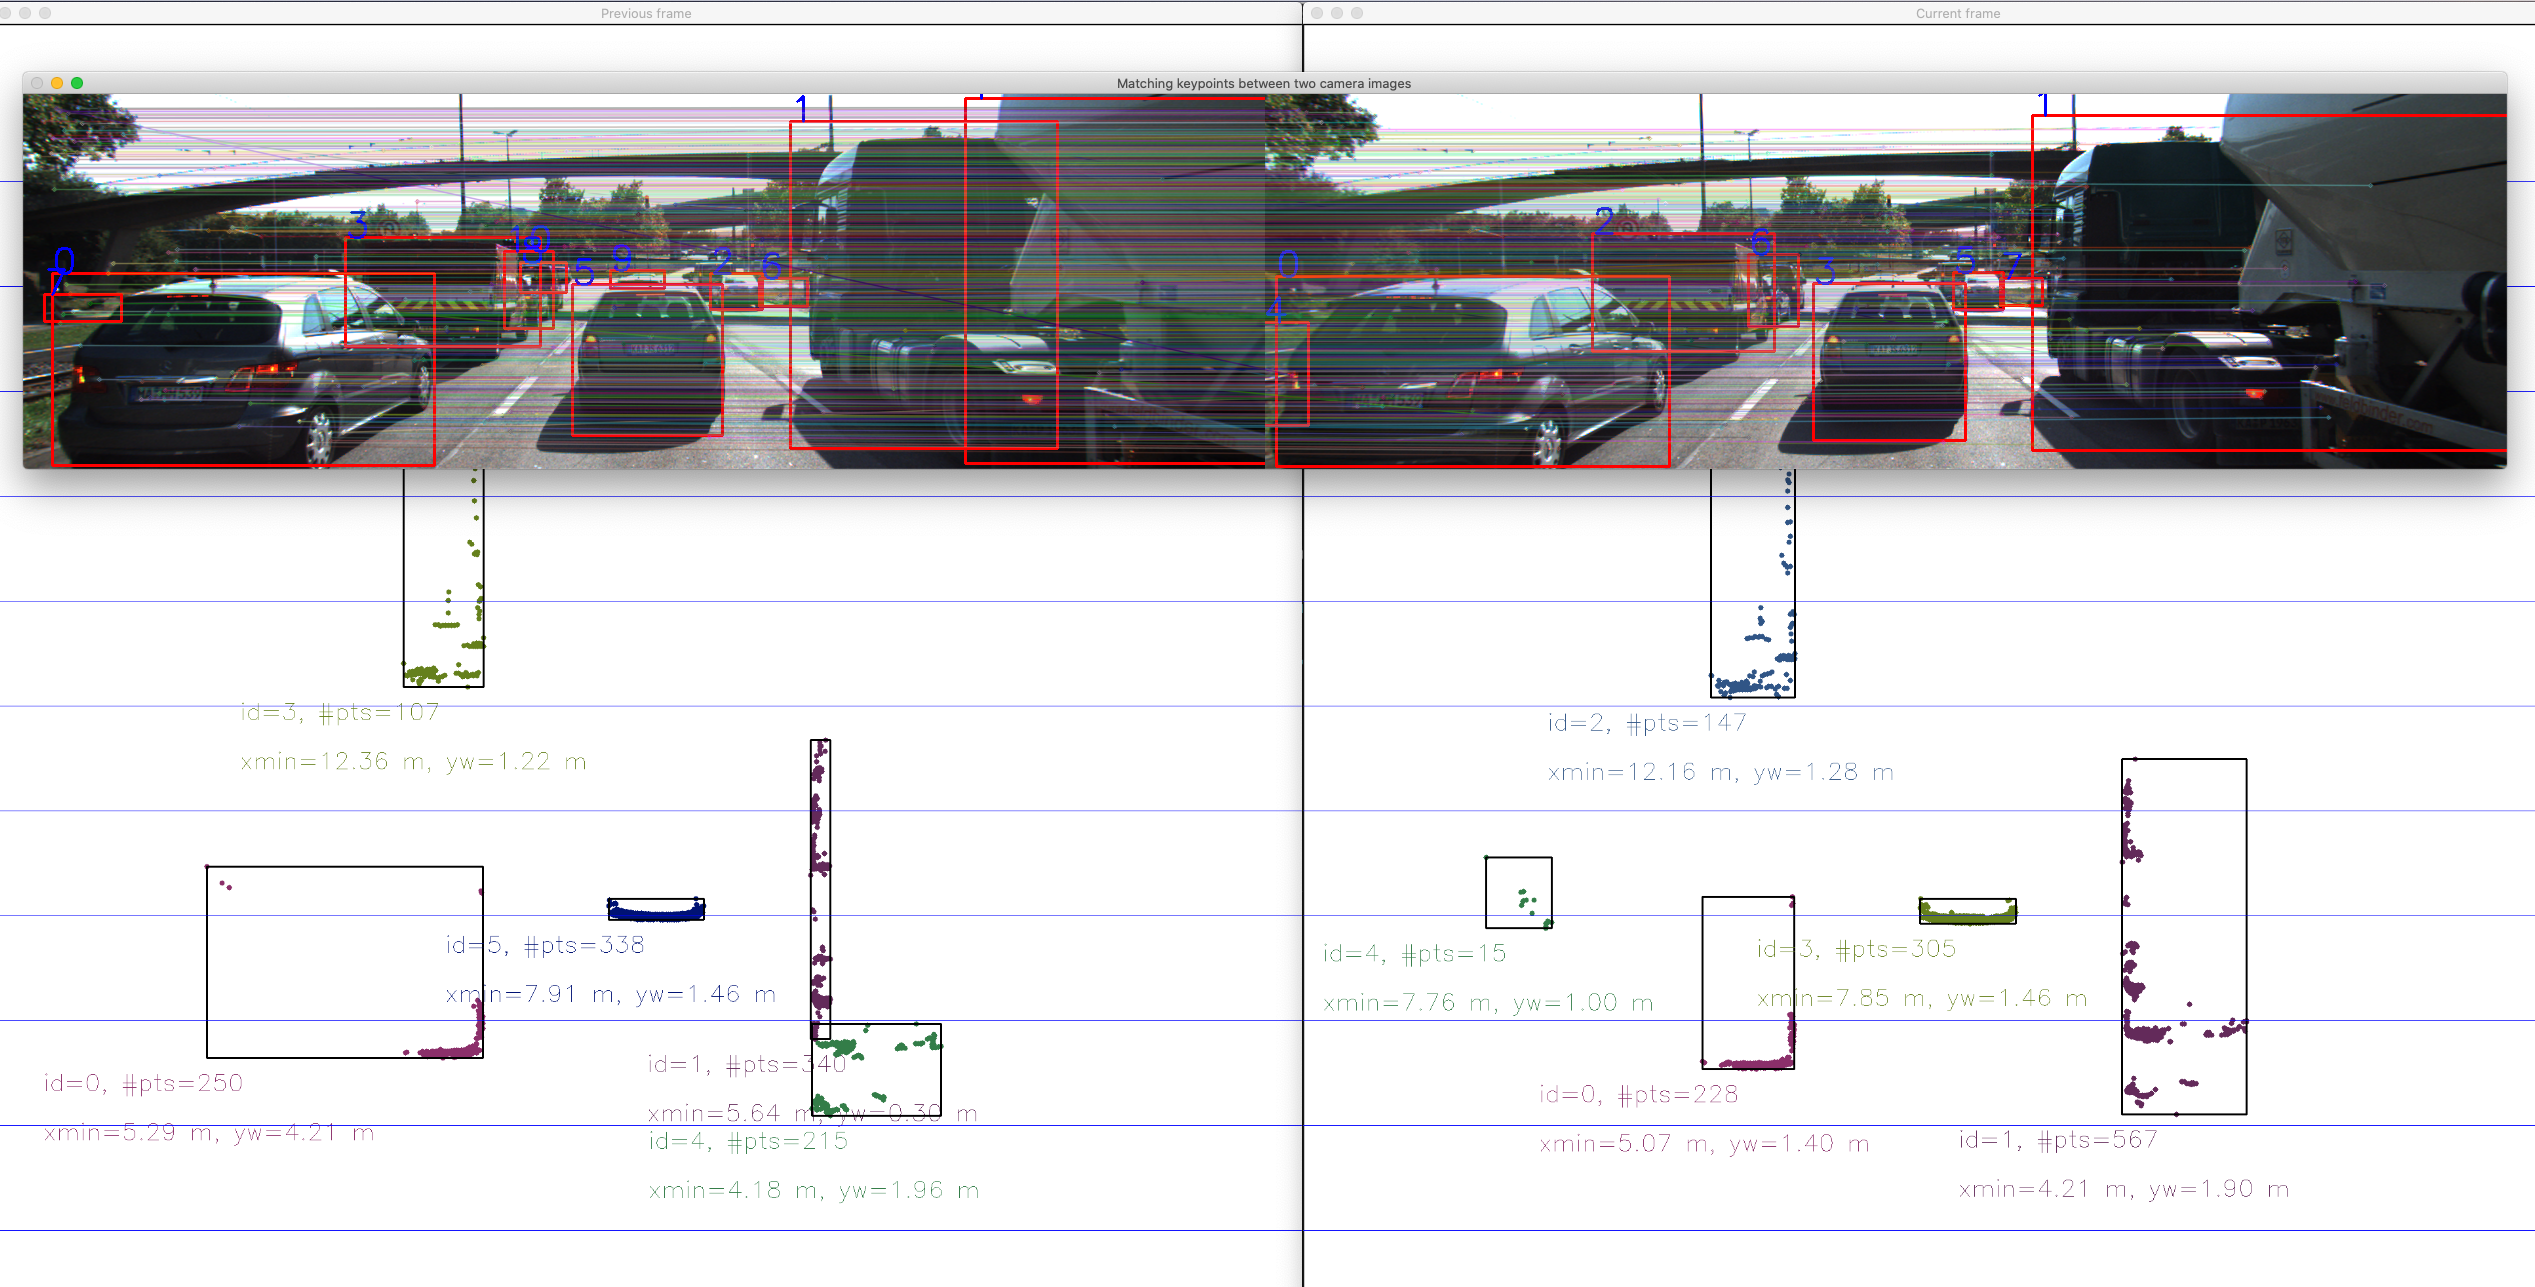
\includegraphics[width=0.8\columnwidth]{./img/3D_object_matching}
	\caption{Simultaneous visualization of the 3D top view from the previous and current frame,
		along with the keypoint descriptor matching, the latter being augmented by the
		2D bounding boxes.
		In this specific scene, the identifier of the leading vehicle changes
		from 5 to 3.}
	\label{fig:matching_3d_objects}
\end{figure}

\section*{FP.2 Compute Lidar-based TTC}
\textcolor{gray}{\textit{Compute the time-to-collision in second for all matched 3D objects using only Lidar measurements from the matched bounding boxes between current and previous frame. }}

According to lesson 2, the time-to-collision (TTC) based on a constant velocity model is
\begin{equation}
\label{eqn:lidar:ttc}
	t_\text{ttc} = \frac{d_1}{v_0} = \frac{d_1 \Delta t}{d_0 - d_1}
\end{equation}
with $d_0$ being the distance from our vehicle to the lead vehicle in the previous frame (index 0),
and $d_1$ being the distance from our vehicle to the lead vehicle in the current frame (index 1).
$v_0$ is the velocity. As it is a constant velocity model, $v_0 = v_1$.
$\Delta t$ is the step size, i.e., the difference between the time stamps of
the individual measurements. $\Delta t$ is the reciprocal of the frame rate.

The current model for the vehicle extent consists of axis-aligned bounding boxes.
In other words, any (non-zero) orientation of the vehicles as well as
curvature on their boundary is neglected.
For this reason, it is valid to assume that the tail of the vehicles can be represented
by a plane with a normal vector which is pointing along the ego vehicle's $x$-axis
($x$ pointing forward in accordance with ISO 8855 and as used throughout this course).
This in turn allows us to use the plane fitting RANSAC from the Lidar course
in order to robustly estimate the tail of the lead vehicle, thereby removing outliers, as
can be seen in Figure~\ref{fig:lidar_ransac}.
I included my Lidar code into the project, slightly adapted for the Camera course data types, in order
to compute the RANSAC. The point cloud library is not needed.

\begin{figure}
	\centering
	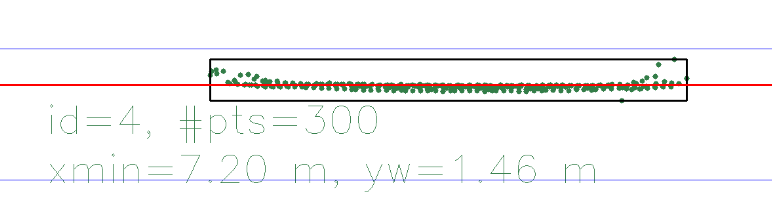
\includegraphics[width=0.8\columnwidth]{./img/lidar_ransac_vehicle_tail}
	\caption{Estimation of the tail of the lead vehicle by means of plane
			fitting using RANSAC. The plane is constrained to have
			a normal vector which is pointing along the $x$-axis.
			In the top view, the red line represents the plane.
			Note how the outlier in the bottom right region enlarges
			the bounding box, but is rejected by the plane fit.}
	\label{fig:lidar_ransac}
\end{figure}


\section*{FP.3 Associate Keypoint Correspondences with Bounding Boxes}
\textcolor{gray}{\textit{Prepare the TTC computation based on camera measurements by associating keypoint correspondences to the bounding boxes which enclose them. All matches which satisfy this condition must be added to a vector in the respective bounding box.}}

First of all, as before,
const correctness is established (not related to the
function though).

As has been recommended by Andreas Haja, I looped over all
keypoint matches and checked if the associated current keypoint
is within the region of interest.
This is a necessary requirement.
It is however not sufficient for a valid keypoint match, as
there might be outliers.
Therefore, as has also been recommended, I computed the
Euclidean distance~$d$ for every keypoint match (in the region of interest).
Based on those distances, I computed the mean~$\mu$ and the
standard deviation~$\sigma$.
A keypoint match is then declared to be valid if
\begin{equation}
	|d - \mu| < 2 \sigma.
\end{equation}
This means that it must not be too far off.

\section*{FP.4 Compute Camera-based TTC}
\textcolor{gray}{\textit{Compute the time-to-collision in second for all matched 3D objects using only keypoint correspondences from the matched bounding boxes between current and previous frame.}}

In order to solve this task, I used the formulas
which have been provided in Lesson 3
(Engineering a Collision Detection System),
Concept 3 (Estimating TTC with a Camera).
I used the keypoints in order to compute an
average distance ratio instead of using the heights,
as has been explained towards the end of that concept.
The TTC formula is
\begin{equation}
	t_\text{ttc} = \frac{- \Delta t}{1 - \rho}
\end{equation}
with $\rho$ being the average distance ratio
between the keypoints of the current frame
and the keypoints of the previous frame.

\section*{FP.5 Performance Evaluation 1}
\textcolor{gray}{\textit{Find examples where the TTC estimate of the Lidar sensor does not seem plausible. Describe your observations and provide a sound argumentation why you think this happened.}}

In order to address this task, I extended my performance evaluation class
from the midterm project so that I can export the Lidar-based distance, velocity,
and TTC estimates.
The values are depicted in Table~\ref{tab:lidar_estimates} and visualized in
Figures~\ref{fig:lidar_distances} to \ref{fig:lidar_ttc}.

It can be seen in Figure~\ref{fig:lidar_distances} that the distances
are located approximately on a straight line.

As we are approaching the leading vehicle, we can expect the TTC to decrease.
I therefore decided to introduce yet another metric: the expected collision time (ECT).
This makes it easier to spot outliers, as the trend has been removed, and
the ECT can be assumed to be constant based on a constant-velocity model.
The ECT is the TTC plus the current time that has passed since the start
of the program. As the frame rate is $10\,\text{Hz}$, we are adding $0.1\,\text{s}$
for every frame that has passed.
The resulting ECT is depicted in Figure~\ref{fig:lidar_ect}, along with the mean
value and the 1-sigma band.
It can be seen that there are 3 points over the 1-sigma band
to the top, and 3 points below the 1-sigma band to the bottom.
I decided to analyze the one at $t=8$ and $t=14$
in detail, as those seem to be the largest ``outliers'' to the top and bottom
respectively.
In can also be seen that the velocity, which is an
essential part for computing the TTC
according to Equation~\ref{eqn:lidar:ttc}, has ``outliers''
at time steps $t=8$ and $t=14$.
The velocity in turn is computed based on the distance
change, so I have a look at the distances, as is also
recommended to do in the course:
\textit{"The assertion that the TTC is off should be based on manually estimating the distance to the rear of the preceding vehicle from a top view perspective of the Lidar points."}

The bird's eye view for the time stamps 7 and 8
is shown in Figure~\ref{fig:lidar_birds_eye_view_1}.
It can be seen that the RANSAC-based distance estimation
is shifted a bit towards the head of the leading
vehicle, therefore decreasing the distance
delta and the velocity estimate, and at the same
time increasing the TTC.

The bird's eye view for the time stamps 13 and 14
is shown in Figure~\ref{fig:lidar_birds_eye_view_2}.
To be honest, I cannot see a geometric reason
caused by the Lidar point cloud which would
cause the RANSAC-based
distance estimate to be ``way off''.
The RANSAC-fitted line is actually moving quite
well with the Lidar point cloud.

Summarizing the task, I did not find any TTC which
deserves to be labelled as ``way off''.
Only the TTC at time stamp $t=8$ is outside the
two $\sigma$ domain and therefore a real outlier.
The other points are within the 2-sigma band of the
associated Gaussian distribution and therefore should not
be called outliers, but rather noise.

However, as required,
I want to give a sound argumentation and
name several reasons why the TTC seems noisy,
and point out avenues how to improve the TTC estimate:
\begin{enumerate}
	\item The constant velocity model does not adequately
		describe the relative velocity between the leading
		vehicle and our vehicle.
		Especially as we are heading towards and intersection
		and therefore decelerating, a constant velocity
		model might be an oversimplification.
		I propose to use a constant acceleration model.
	\item We compute the velocity directly by
		evaluating the delta between the distance~$d_1$
		of the previous frame and the distance~$d_0$
		of the current frame.
		That makes the velocity highly susceptible to noise.
		A better approach would be to use some kind of
		low-pass filter
		(realized as IIR or FIR filter) in order to smoothen the
		velocity and TTC signals, or alternatively
		to use a Kalman filter on top of our
		constant velocity (or constant acceleration)
		motion model.
	\item A geometric reasoning:
		Neither a bounding box nor a line fit
		(as done using RANSAC here) is not a perfect model
		for the shape of the leading vehicle, as its
		tail is not flat.
		It might prove beneficial to fit an ellipse
		segment instead, as this better describes the
		shape of the leading vehicle's tail.
\end{enumerate}



\begin{table}
	\centering
	\caption{Lidar-based distance, velocity, and TTC estimates.}
	\label{tab:lidar_estimates}
	\begin{tabular}{l|rrr}
Time index & Distance (m) & Velocity (m/s) & TTC (s) \\ \hline
0       & 8.015 & 0.549994  & 14.5729 \\
1       & 7.945 & 0.709996  & 11.1902 \\
2       & 7.900 & 0.489998  & 16.1225 \\
3       & 7.843 & 0.590000  & 13.2932 \\
4       & 7.774 & 0.689998  & 11.2667 \\
5       & 7.724 & 0.660000  & 11.7030 \\
6       & 7.653 & 0.730000  & 10.4836 \\
7       & 7.606 & 0.469999  & 16.1830 \\
8       & 7.565 & 0.419998  & 18.0120 \\
9       & 7.510 & 0.579996  & 12.9484 \\
10      & 7.436 & 0.710001  & 10.4732 \\
11      & 7.370 & 0.660000  & 11.1667 \\
12      & 7.290 & 0.809999  & 9.00002 \\
13      & 7.229 & 0.619998  & 11.6597 \\
14      & 7.140 & 0.890002  & 8.02245 \\
15      & 7.062 & 0.730004  & 9.67392 \\
16      & 6.974 & 0.869999  & 8.01610 \\
17      & 6.910 & 0.500002  & 13.8199
	\end{tabular}
\end{table}

\begin{figure}
	\centering
	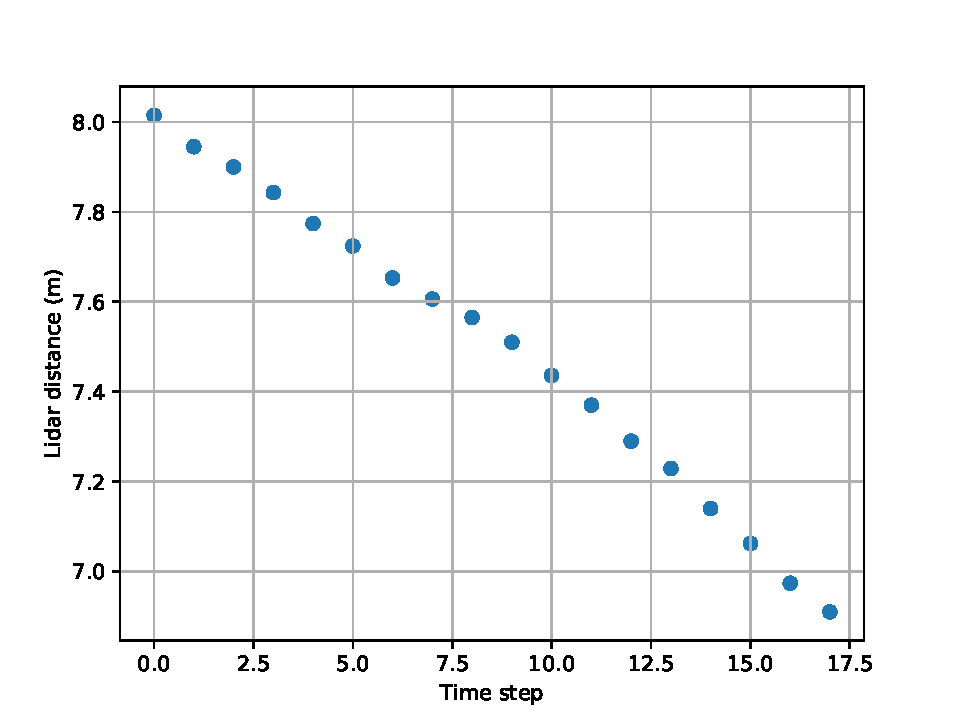
\includegraphics[width=0.8\columnwidth]{./img/lidar_distances}
	\caption{Lidar distance over time. The time is given in time steps
			(not in seconds).}
	\label{fig:lidar_distances}
\end{figure}

\begin{figure}
	\centering
	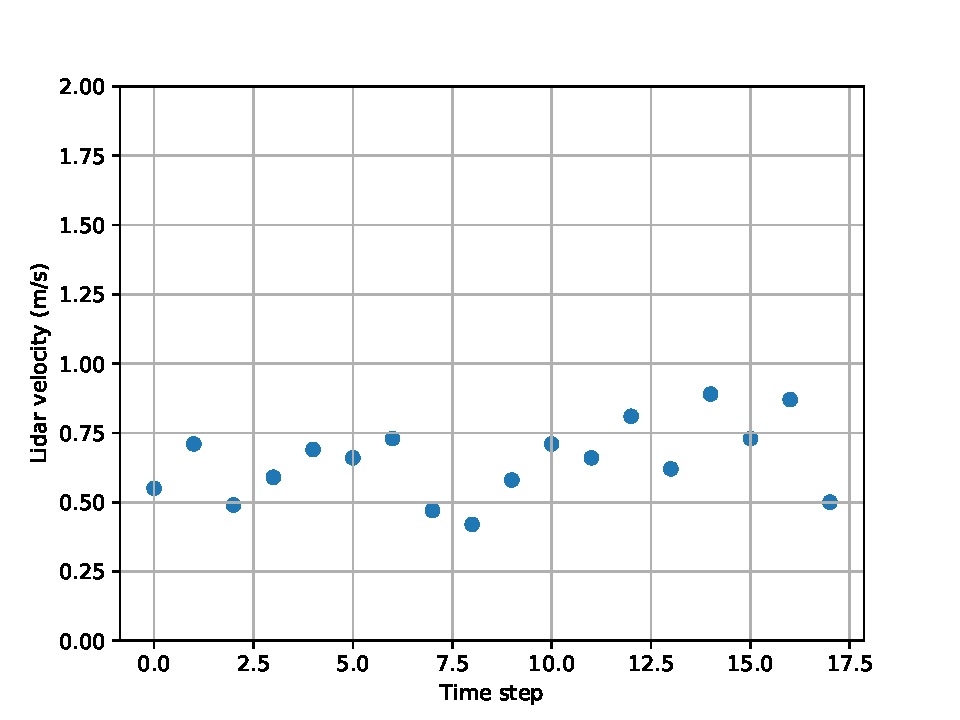
\includegraphics[width=0.8\columnwidth]{./img/lidar_velocities}
	\caption{Lidar velocity over time. The time is given in time steps
			(not in seconds).}
	\label{fig:lidar_velocities}
\end{figure}

\begin{figure}
	\centering
	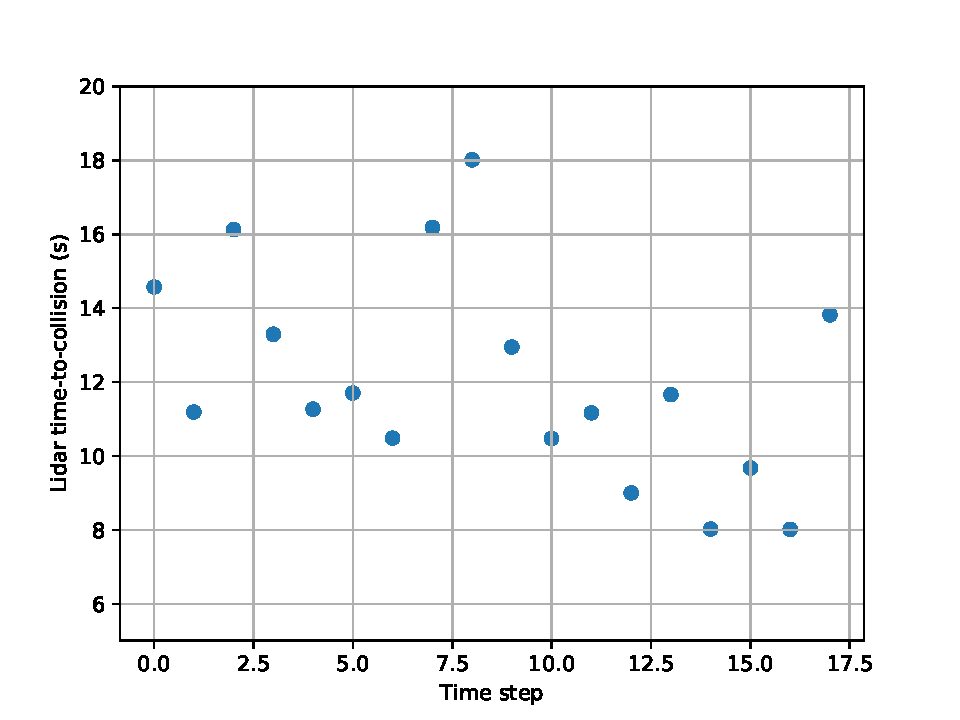
\includegraphics[width=0.8\columnwidth]{./img/lidar_ttc}
	\caption{Lidar-based time-to-collision. The time is given in time steps
			(not in seconds).}
	\label{fig:lidar_ttc}
\end{figure}

\begin{figure}
	\centering
	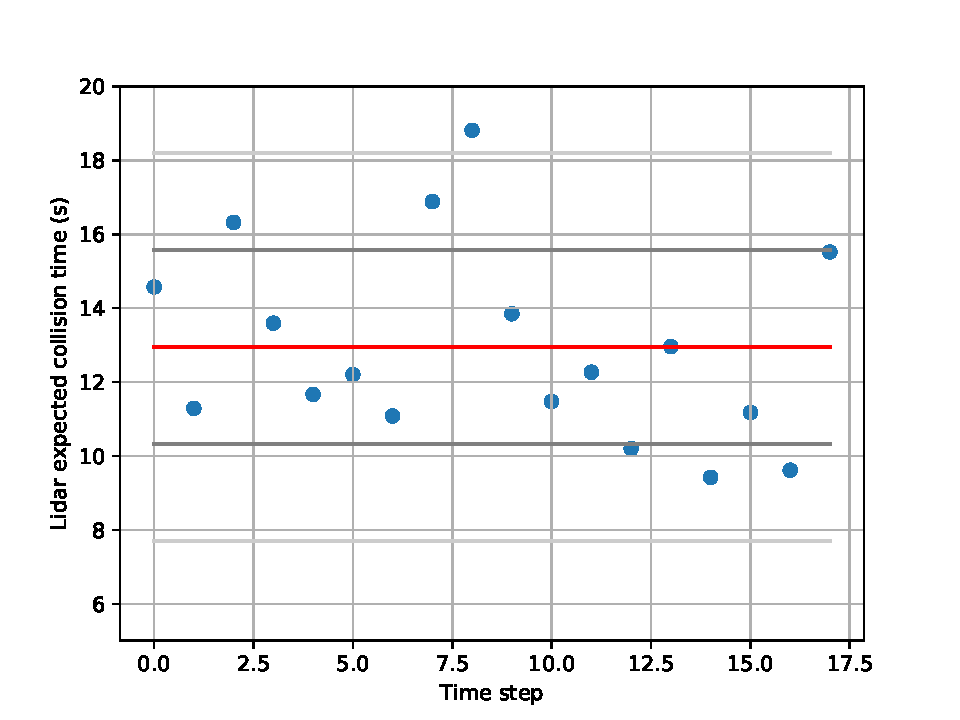
\includegraphics[width=0.8\columnwidth]{./img/lidar_ect}
	\caption{Lidar-based expected collision time. The time is given in time steps
			(not in seconds).
			The red line shows the mean value, and the gray lines
			show the plus/minus one (dark gray) or two (light gray)
			$\sigma$ (standard deviation)
			boundaries.}
	\label{fig:lidar_ect}
\end{figure}

\begin{figure}
	\centering
	\begin{subfigure}[c]{0.45\columnwidth}
		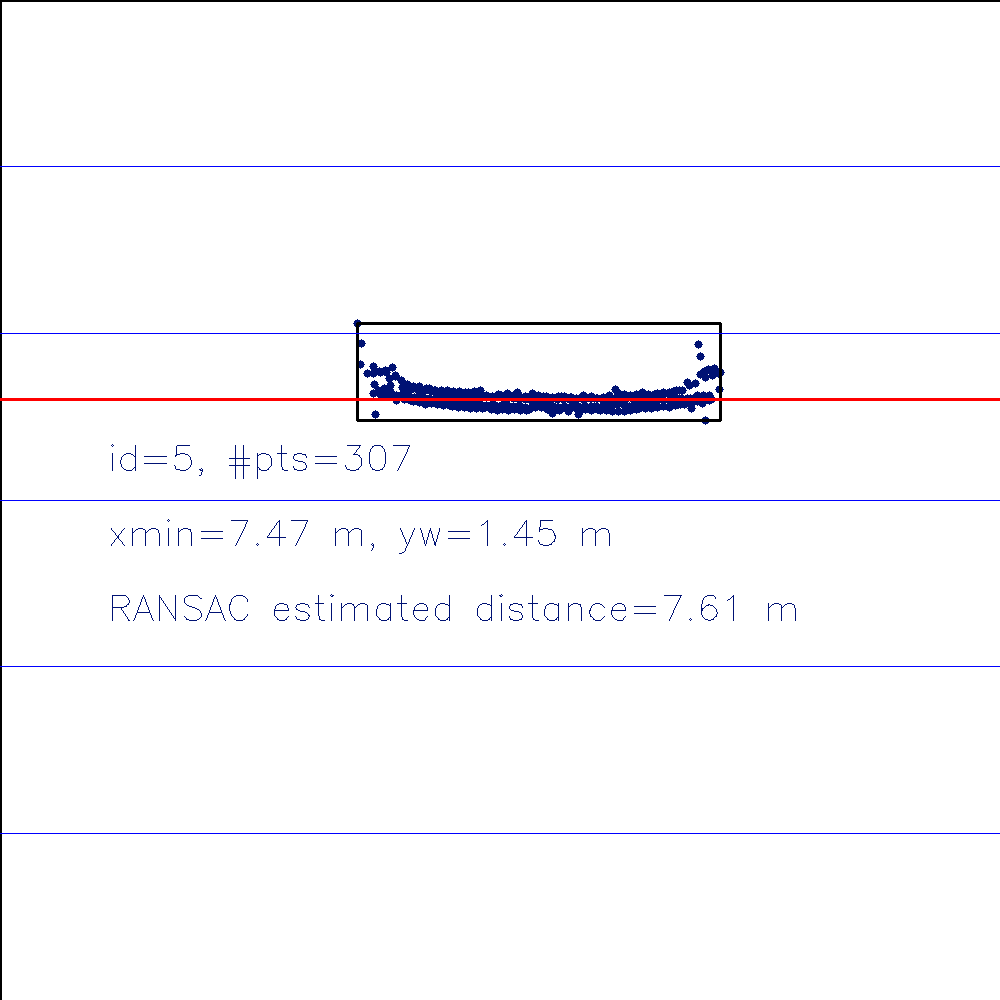
\includegraphics[width=0.8\textwidth]{%
			./performance_eval_lidar/lidar_distance_07}
		\subcaption{Time step 7.}
	\end{subfigure}
	\begin{subfigure}[c]{0.45\columnwidth}
		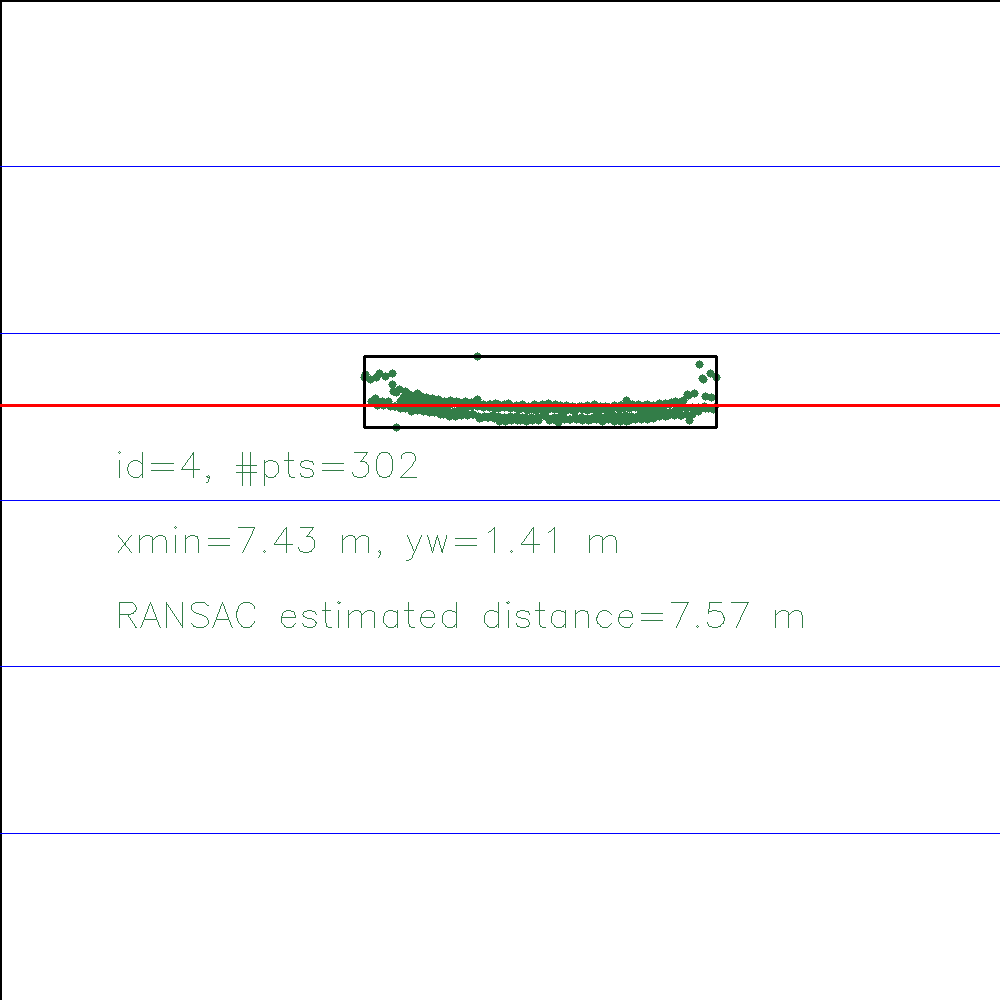
\includegraphics[width=0.8\textwidth]{%
			./performance_eval_lidar/lidar_distance_08}
		\subcaption{Time step 8.}
	\end{subfigure}
	\caption{Lidar distances bird's eye view.
			The distance between the blue horizontal
			lines corresponds to one meter.
			The world view starts at $x=4\,\text{m}$
			and ends at $x=10\,\text{m}$.}
	\label{fig:lidar_birds_eye_view_1}
\end{figure}

\begin{figure}
	\centering
	\begin{subfigure}[c]{0.45\columnwidth}
		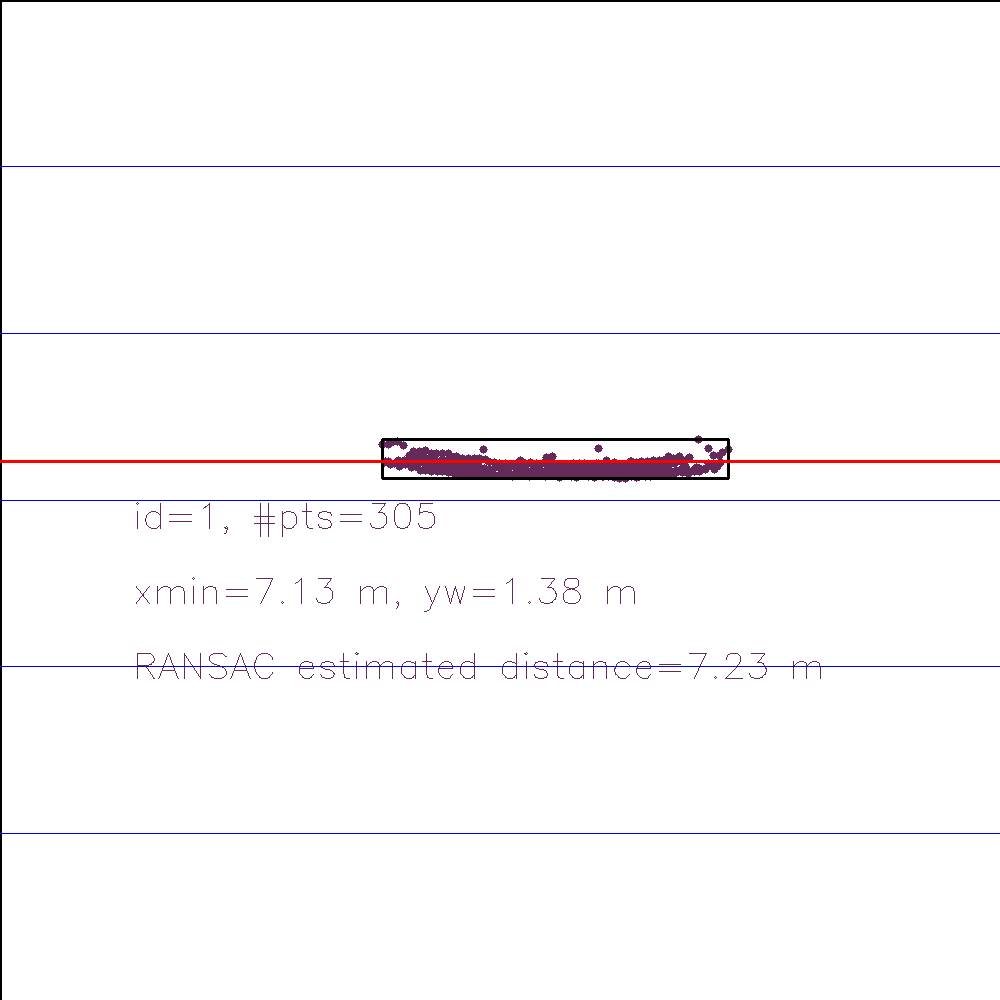
\includegraphics[width=0.8\textwidth]{%
			./performance_eval_lidar/lidar_distance_13}
		\subcaption{Time step 13.}
	\end{subfigure}
	\begin{subfigure}[c]{0.45\columnwidth}
		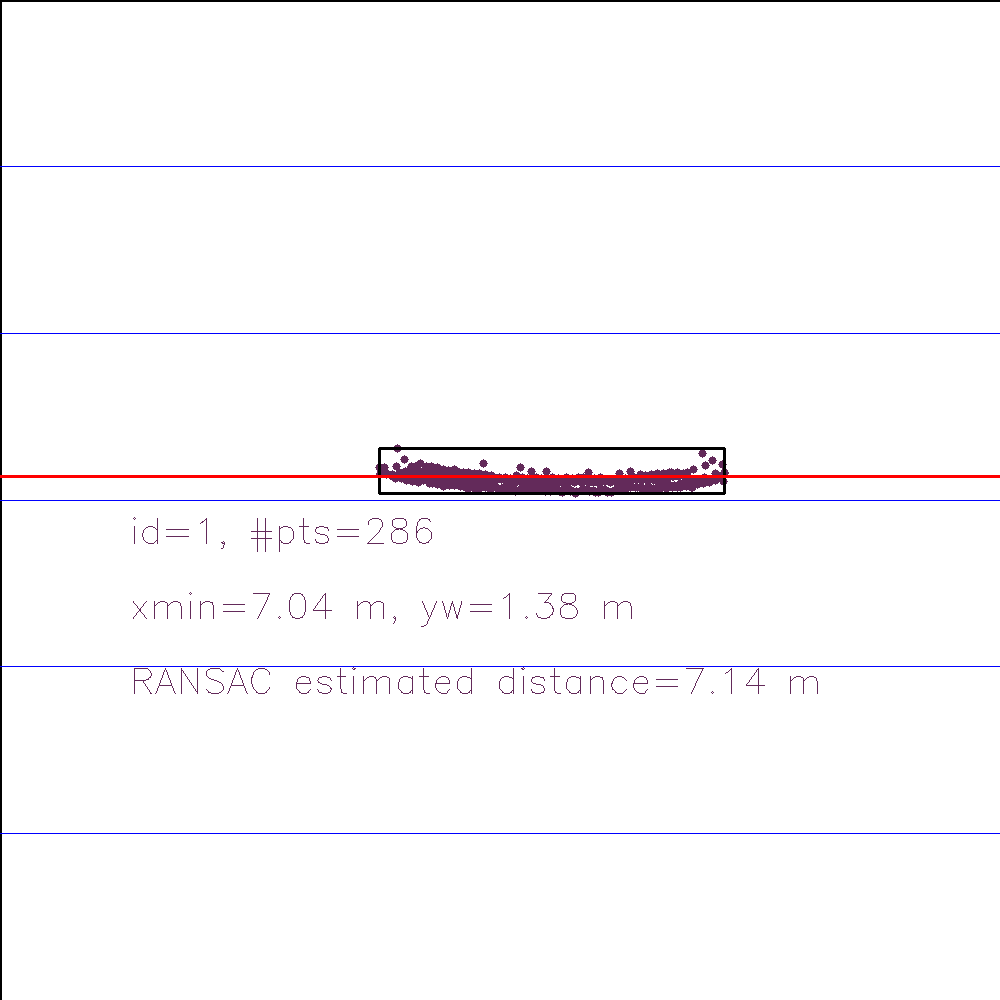
\includegraphics[width=0.8\textwidth]{%
			./performance_eval_lidar/lidar_distance_14}
		\subcaption{Time step 14.}
	\end{subfigure}
	\caption{Lidar distances bird's eye view.
			The distance between the blue horizontal
			lines corresponds to one meter.
			The world view starts at $x=4\,\text{m}$
			and ends at $x=10\,\text{m}$.}
	\label{fig:lidar_birds_eye_view_2}
\end{figure}

\clearpage

\section*{FP.6 Performance Evaluation 2}
\textcolor{gray}{\textit{Run several detector / descriptor combinations and look at the differences in TTC estimation. Find out which methods perform best and also include several examples where camera-based TTC estimation is way off. As with Lidar, describe your observations again and also look into potential reasons.}}

In order to address this task, I create plots
for the TTC and for the ECT (expected collision time)
for all detector and descriptor combinations.
As in the previous section, the ECT is used because
it does not contain the decreasing trend that we see in the TTC
due to us approaching the leading vehicle,
but rather should be a constant value.

The TTC plots are shown in Figures~\ref{fig:camera:ttc:detector_SHITOMASI}
to \ref{fig:camera:ttc:detector_SIFT}.

I also compute the expected collision time
mean and the standard deviation for
every keypoint detector and descriptor combination.
The smaller the standard deviation the better.
The results are shown in Table~\ref{tab:camera:etc_mean_and_std}.

It can be seen that --opposed to Lidar-- there are now really some TTC estimates
which deserve to be called ``way off''.
One example would be the combination of the Shi-Tomasi detector with
the BRIEF descriptor at time step 6. It can be seen that the TTC is even
estimated to be negative.
An example where the TTC is estimated way too large is the Harris detector
in combination with the BRISK descriptor at time step 12.

Based on the standard deviation, I would recommend to use for instance
\begin{itemize}
	\item Shi-Tomasi detector with BRISK descriptor,
	\item Shi-Tomasi detector with BRIEF descriptor,
	\item Shi-Tomasi detector with SIFT descriptor, or
	\item AKAZE detector with SIFT descriptor.
\end{itemize}
However, even then, the use of some low-pass filter or (model-based)
Kalman filter would be recommended.

% TTC plots
\begin{figure}
	\centering
	\begin{subfigure}[c]{0.45\columnwidth}
		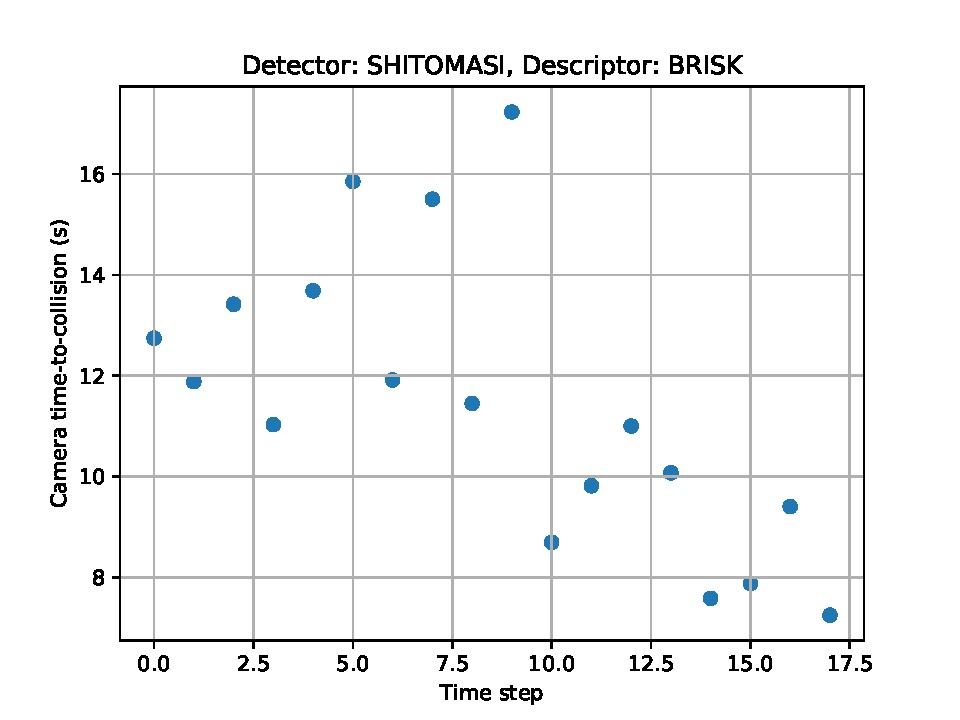
\includegraphics[width=\textwidth]{%
			./img/camera_ttc_det_SHITOMASI_desc_BRISK}
	\end{subfigure}
	\begin{subfigure}[c]{0.45\columnwidth}
		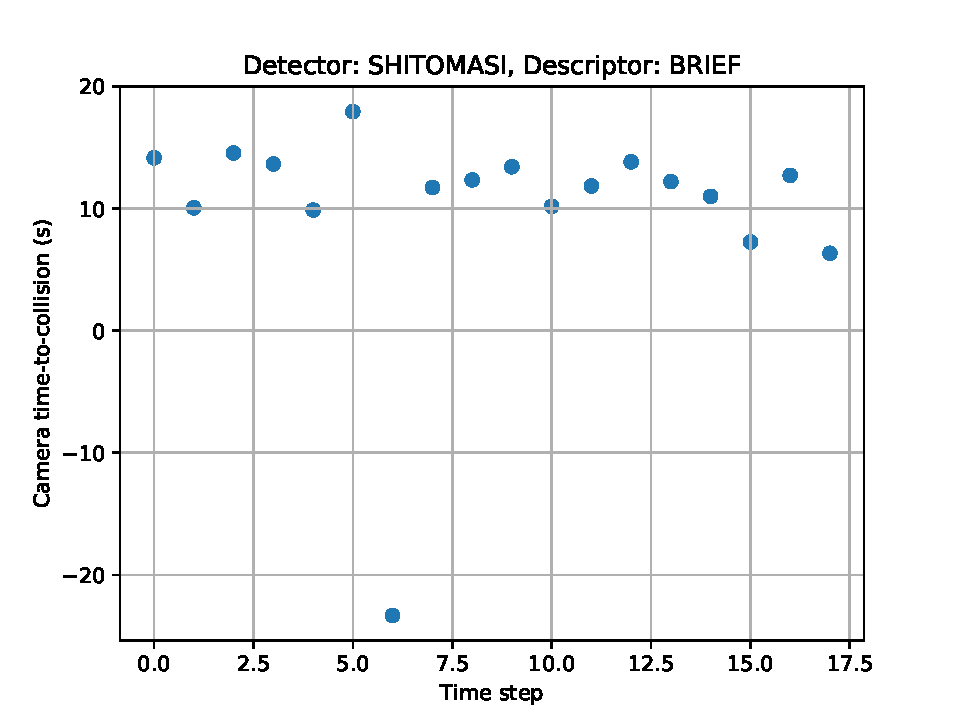
\includegraphics[width=\textwidth]{%
			./img/camera_ttc_det_SHITOMASI_desc_BRIEF}
	\end{subfigure}
	\begin{subfigure}[c]{0.45\columnwidth}
		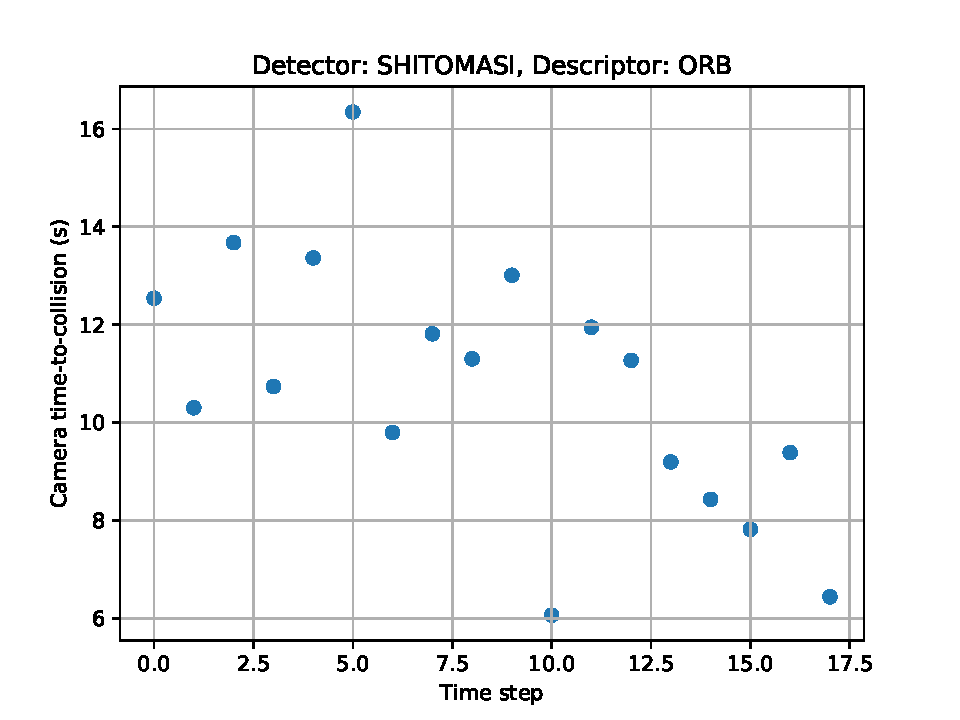
\includegraphics[width=\textwidth]{%
			./img/camera_ttc_det_SHITOMASI_desc_ORB}
	\end{subfigure}
	\begin{subfigure}[c]{0.45\columnwidth}
		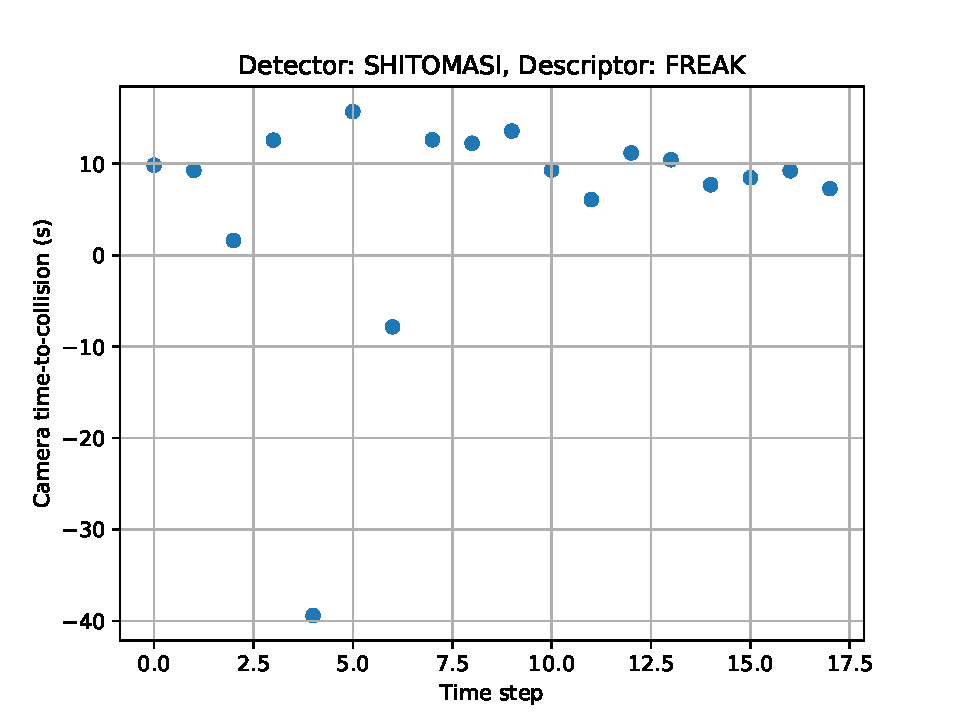
\includegraphics[width=\textwidth]{%
			./img/camera_ttc_det_SHITOMASI_desc_FREAK}
	\end{subfigure}
	\begin{subfigure}[c]{0.45\columnwidth}
		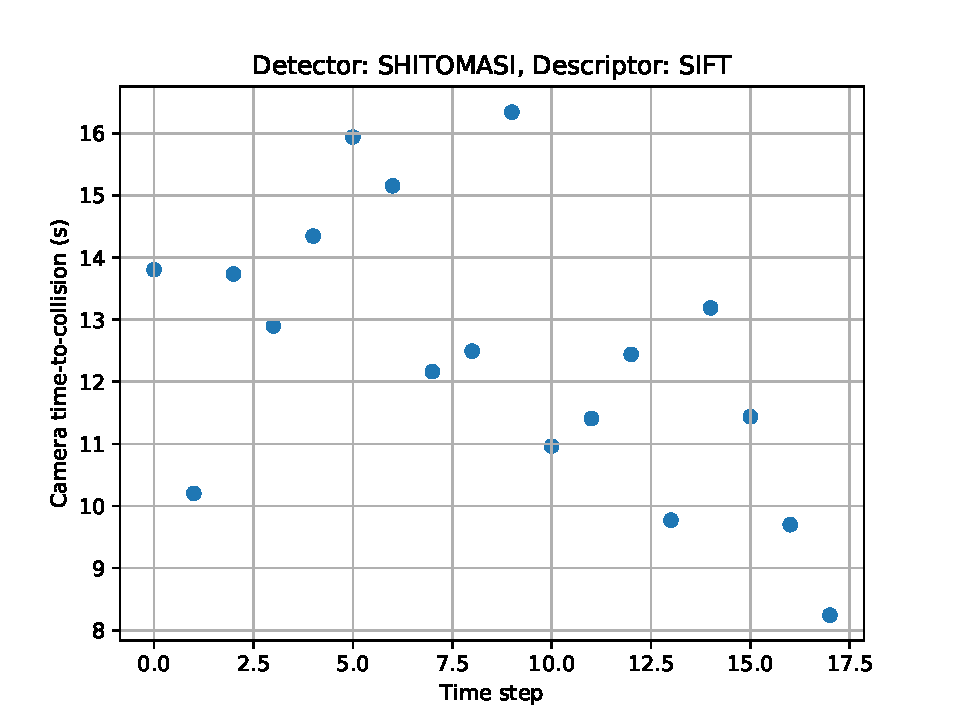
\includegraphics[width=\textwidth]{%
			./img/camera_ttc_det_SHITOMASI_desc_SIFT}
	\end{subfigure}
	\caption{Camera TTC for the Shi-Tomasi detector.}
	\label{fig:camera:ttc:detector_SHITOMASI}
\end{figure}

\begin{figure}
	\centering
	\begin{subfigure}[c]{0.45\columnwidth}
		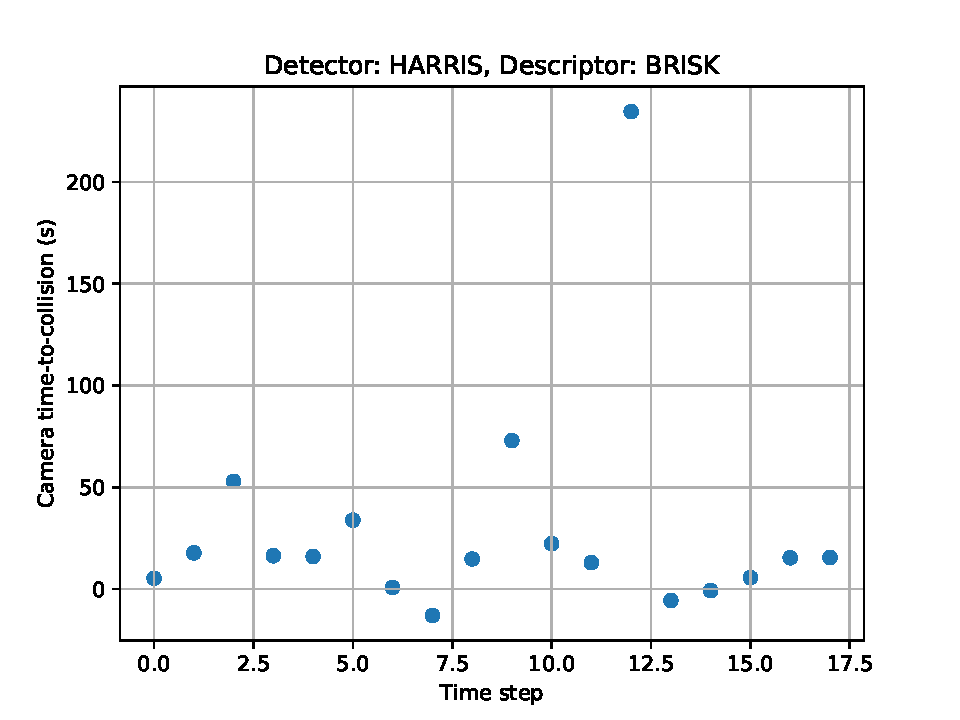
\includegraphics[width=\textwidth]{%
			./img/camera_ttc_det_HARRIS_desc_BRISK}
	\end{subfigure}
	\begin{subfigure}[c]{0.45\columnwidth}
		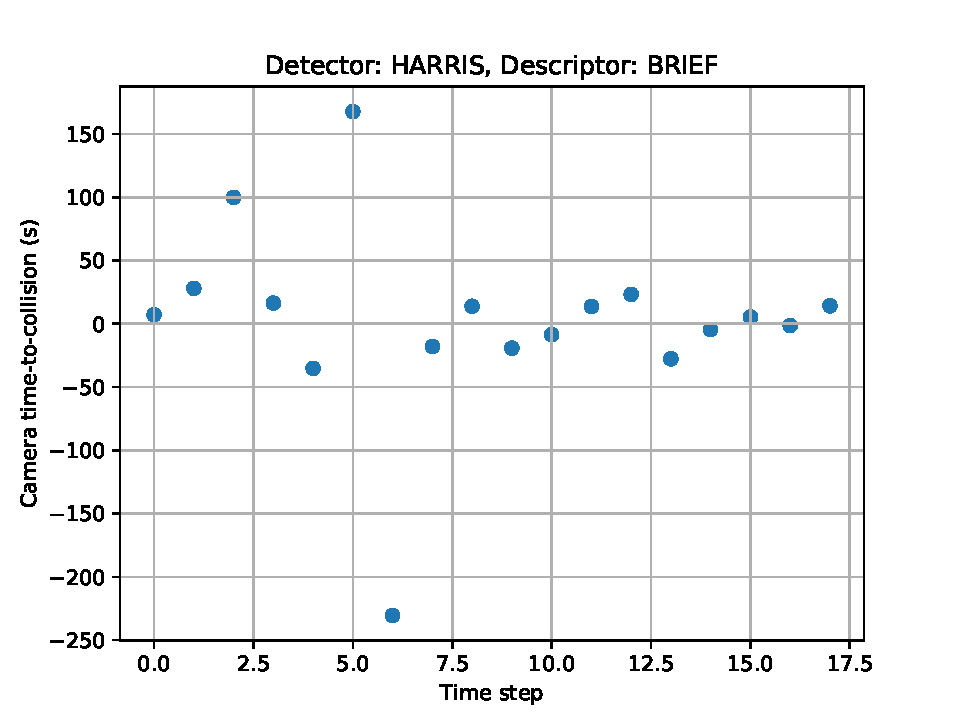
\includegraphics[width=\textwidth]{%
			./img/camera_ttc_det_HARRIS_desc_BRIEF}
	\end{subfigure}
	\begin{subfigure}[c]{0.45\columnwidth}
		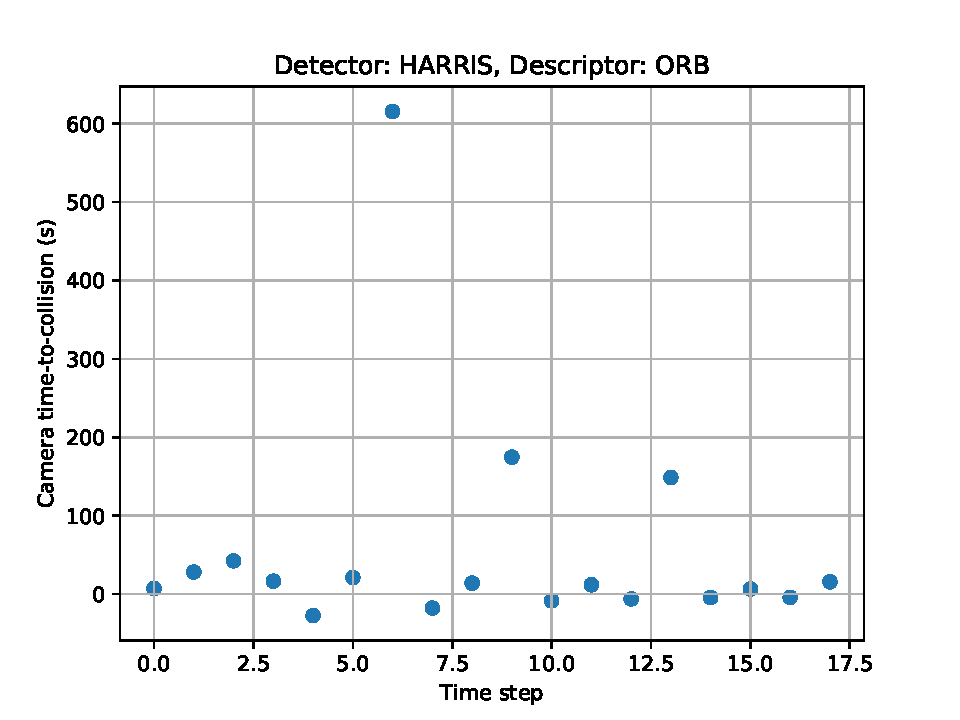
\includegraphics[width=\textwidth]{%
			./img/camera_ttc_det_HARRIS_desc_ORB}
	\end{subfigure}
	\begin{subfigure}[c]{0.45\columnwidth}
		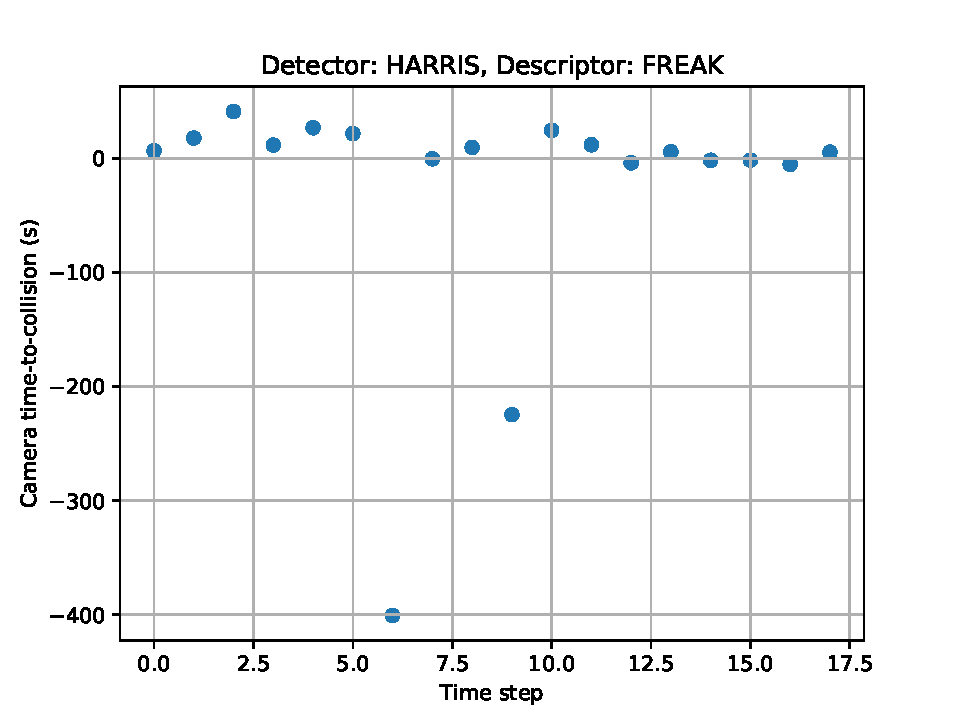
\includegraphics[width=\textwidth]{%
			./img/camera_ttc_det_HARRIS_desc_FREAK}
	\end{subfigure}
	\begin{subfigure}[c]{0.45\columnwidth}
		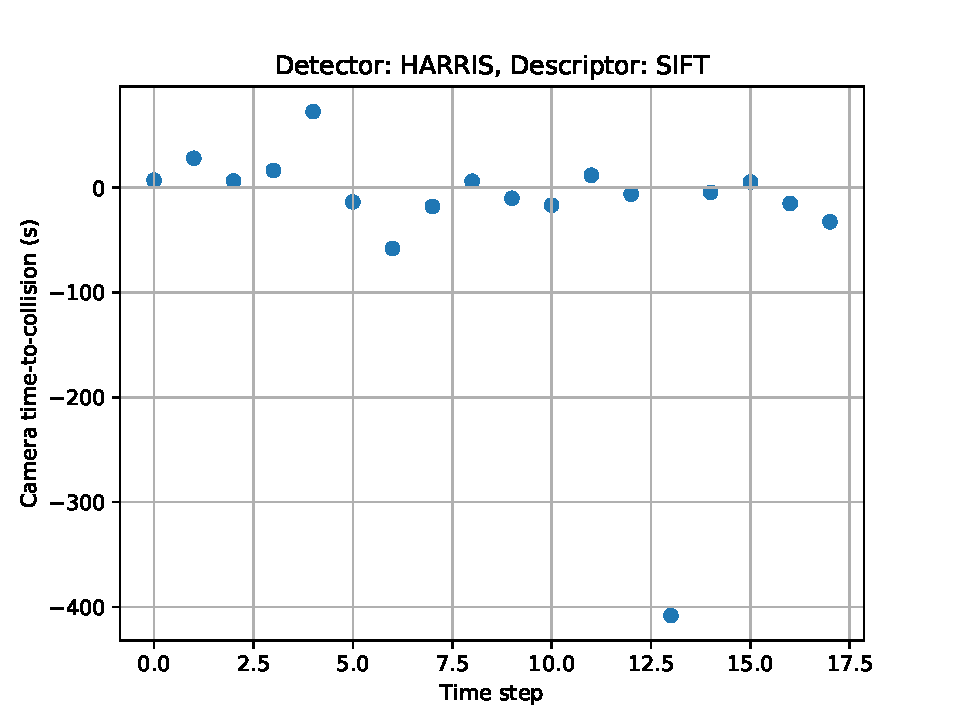
\includegraphics[width=\textwidth]{%
			./img/camera_ttc_det_HARRIS_desc_SIFT}
	\end{subfigure}
	\caption{Camera TTC for the Harris detector.}
	\label{fig:camera:ttc:detector_HARRIS}
\end{figure}

\begin{figure}
	\centering
	\begin{subfigure}[c]{0.45\columnwidth}
		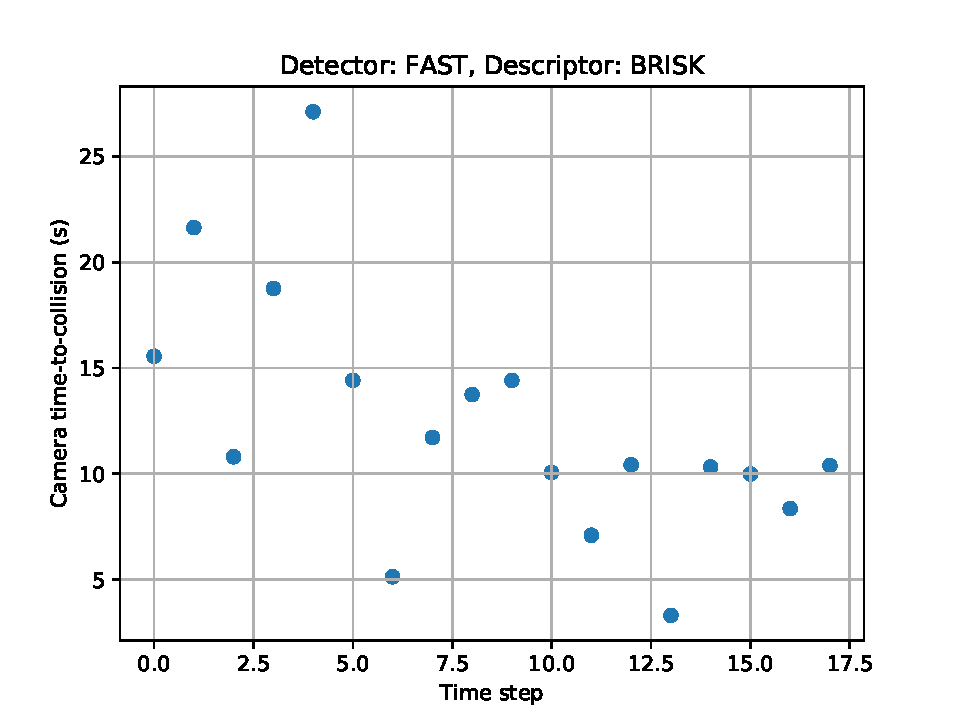
\includegraphics[width=\textwidth]{%
			./img/camera_ttc_det_FAST_desc_BRISK}
	\end{subfigure}
	\begin{subfigure}[c]{0.45\columnwidth}
		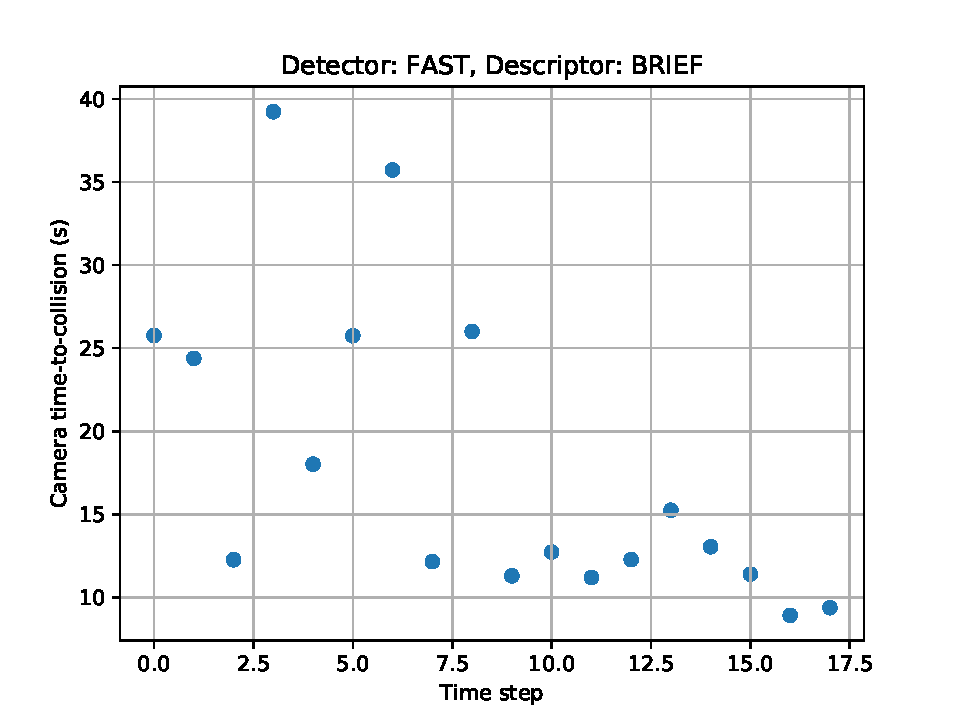
\includegraphics[width=\textwidth]{%
			./img/camera_ttc_det_FAST_desc_BRIEF}
	\end{subfigure}
	\begin{subfigure}[c]{0.45\columnwidth}
		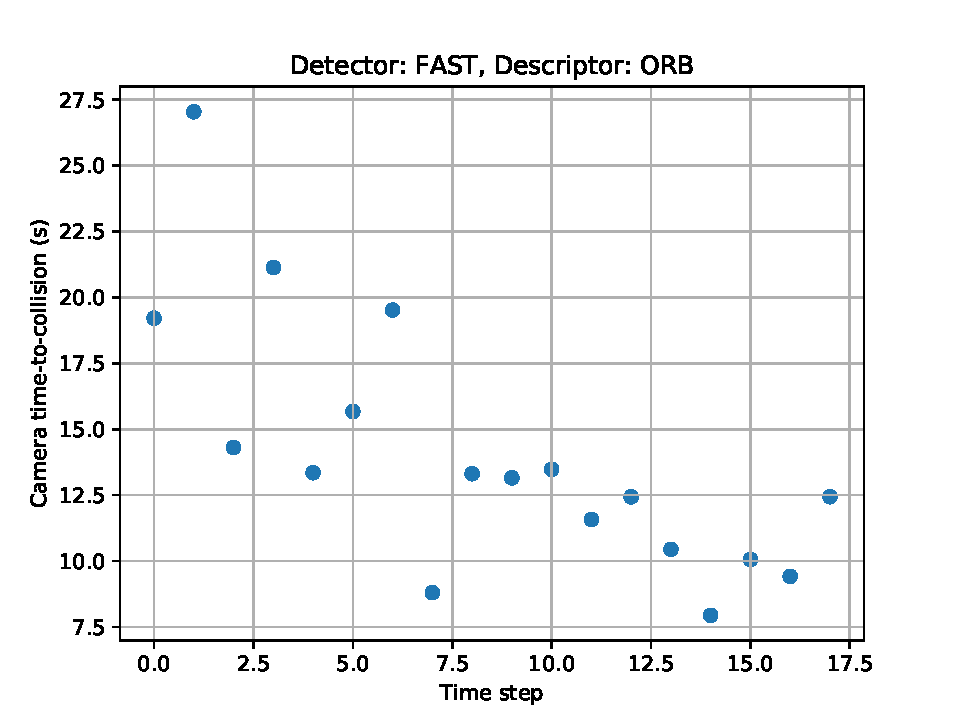
\includegraphics[width=\textwidth]{%
			./img/camera_ttc_det_FAST_desc_ORB}
	\end{subfigure}
	\begin{subfigure}[c]{0.45\columnwidth}
		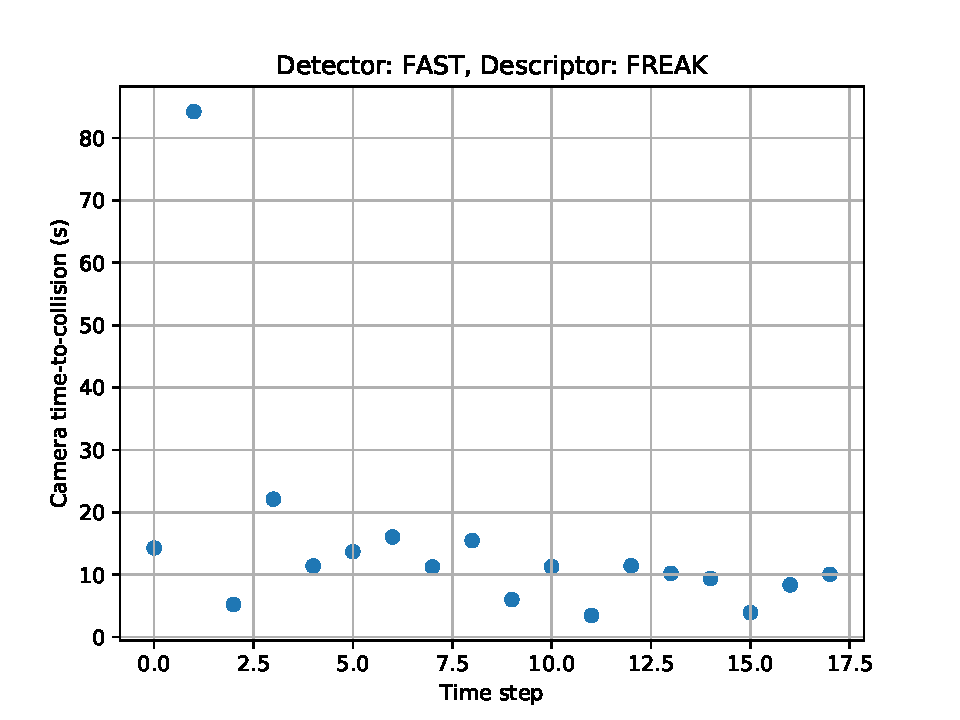
\includegraphics[width=\textwidth]{%
			./img/camera_ttc_det_FAST_desc_FREAK}
	\end{subfigure}
	\begin{subfigure}[c]{0.45\columnwidth}
		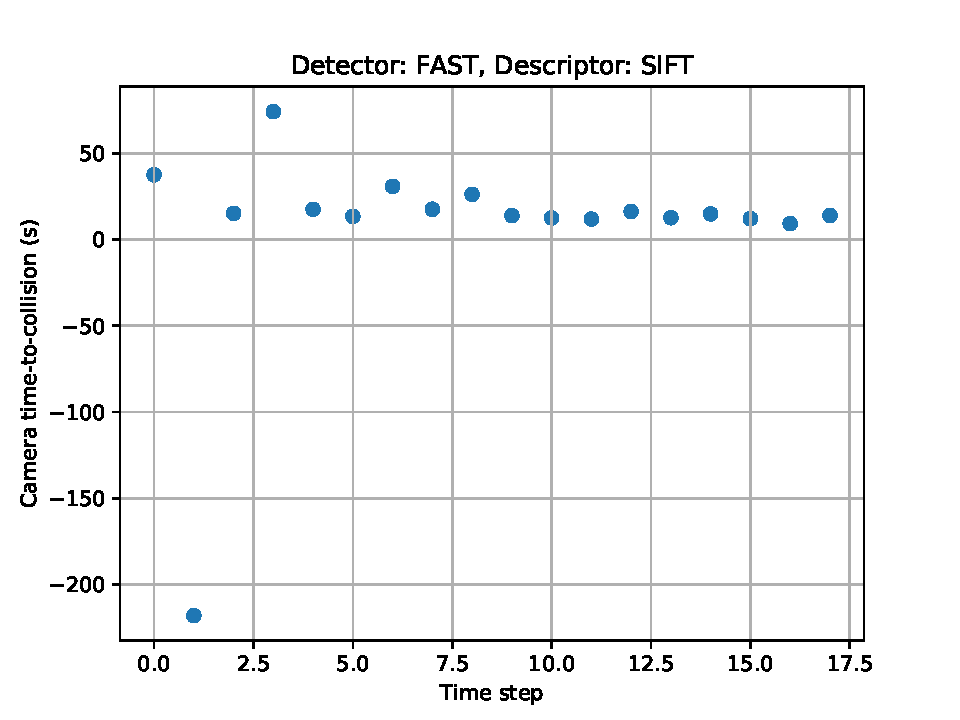
\includegraphics[width=\textwidth]{%
			./img/camera_ttc_det_FAST_desc_SIFT}
	\end{subfigure}
	\caption{Camera TTC for the FAST detector.}
	\label{fig:camera:ttc:detector_FAST}
\end{figure}

\begin{figure}
	\centering
	\begin{subfigure}[c]{0.45\columnwidth}
		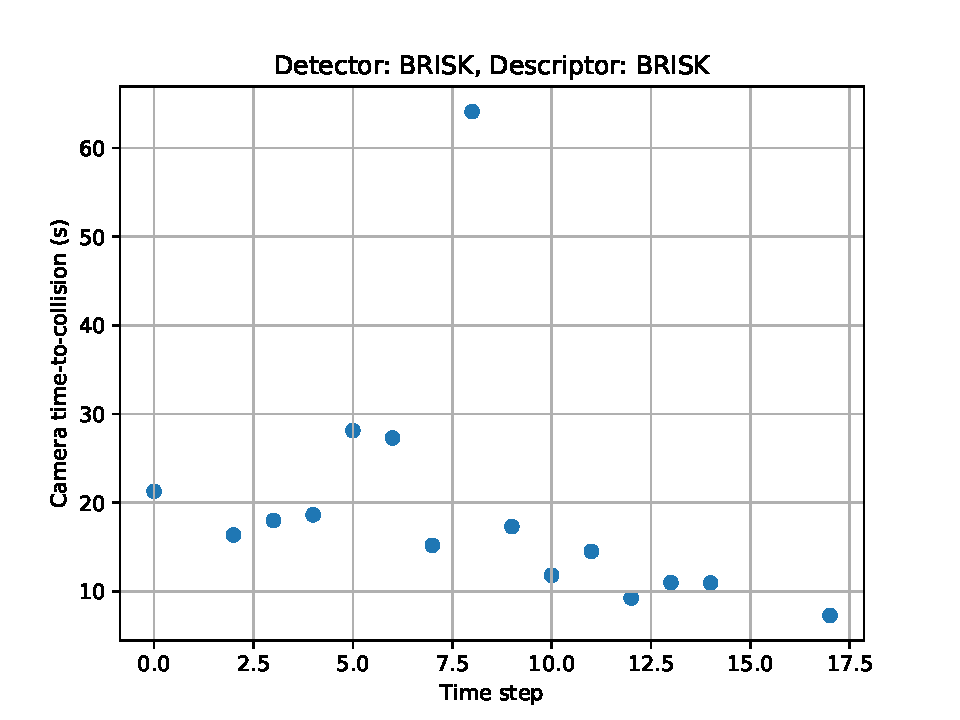
\includegraphics[width=\textwidth]{%
			./img/camera_ttc_det_BRISK_desc_BRISK}
	\end{subfigure}
	\begin{subfigure}[c]{0.45\columnwidth}
		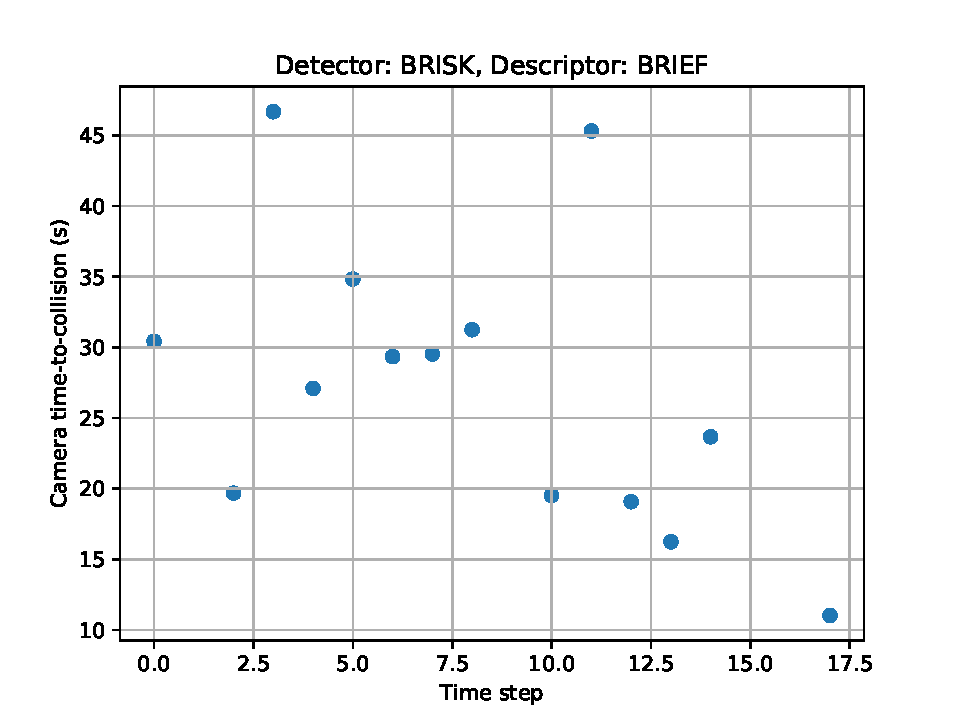
\includegraphics[width=\textwidth]{%
			./img/camera_ttc_det_BRISK_desc_BRIEF}
	\end{subfigure}
	\begin{subfigure}[c]{0.45\columnwidth}
		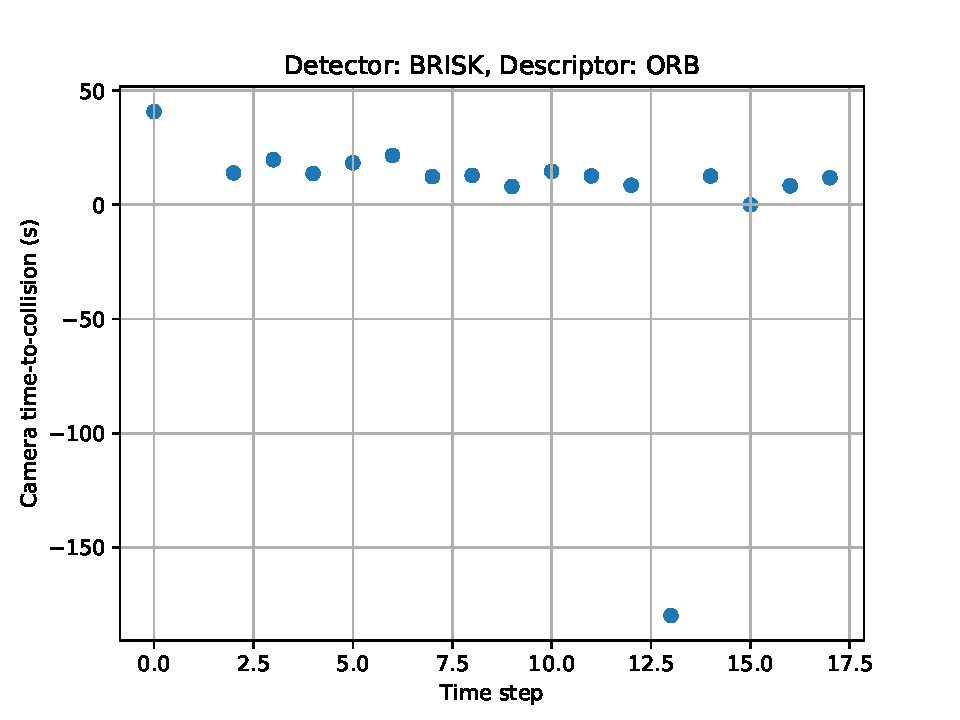
\includegraphics[width=\textwidth]{%
			./img/camera_ttc_det_BRISK_desc_ORB}
	\end{subfigure}
	\begin{subfigure}[c]{0.45\columnwidth}
		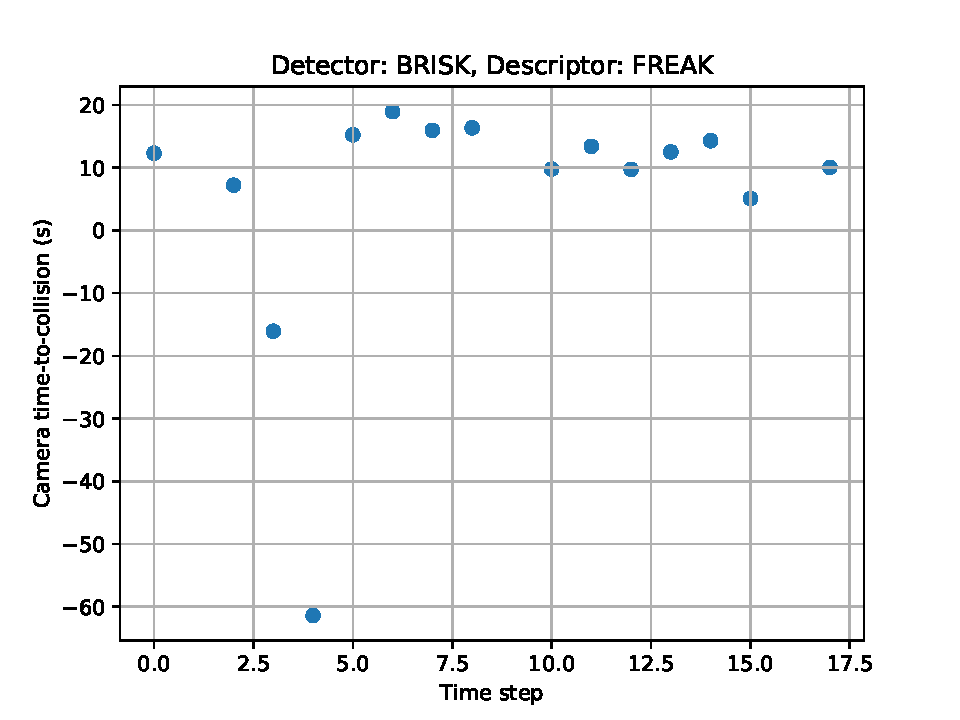
\includegraphics[width=\textwidth]{%
			./img/camera_ttc_det_BRISK_desc_FREAK}
	\end{subfigure}
	\begin{subfigure}[c]{0.45\columnwidth}
		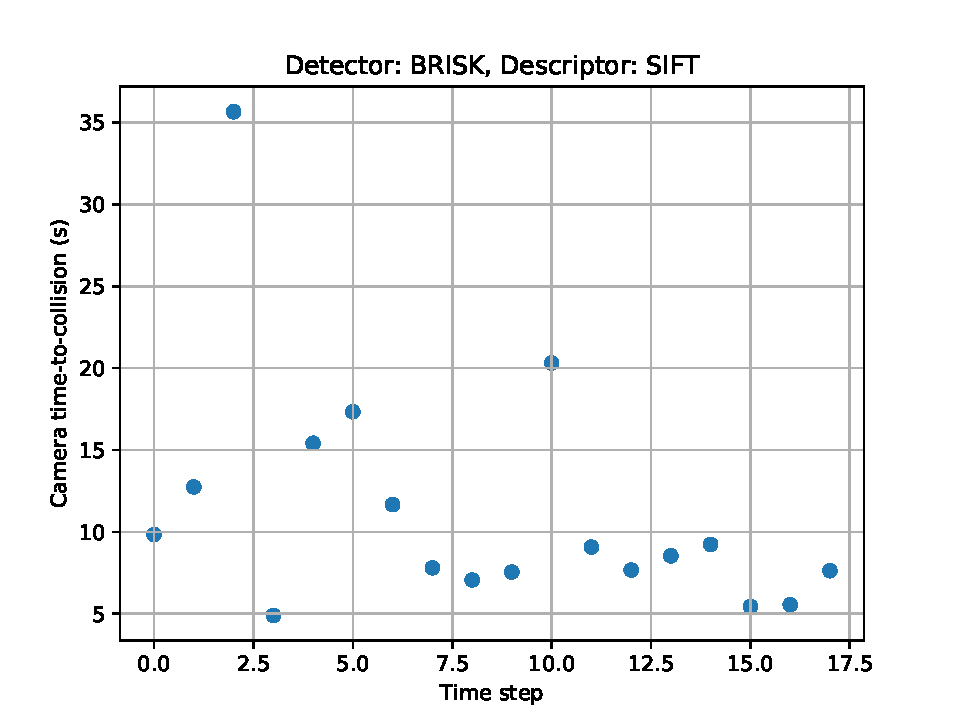
\includegraphics[width=\textwidth]{%
			./img/camera_ttc_det_BRISK_desc_SIFT}
	\end{subfigure}
	\caption{Camera TTC for the BRISK detector.}
	\label{fig:camera:ttc:detector_BRISK}
\end{figure}

\begin{figure}
	\centering
	\begin{subfigure}[c]{0.45\columnwidth}
		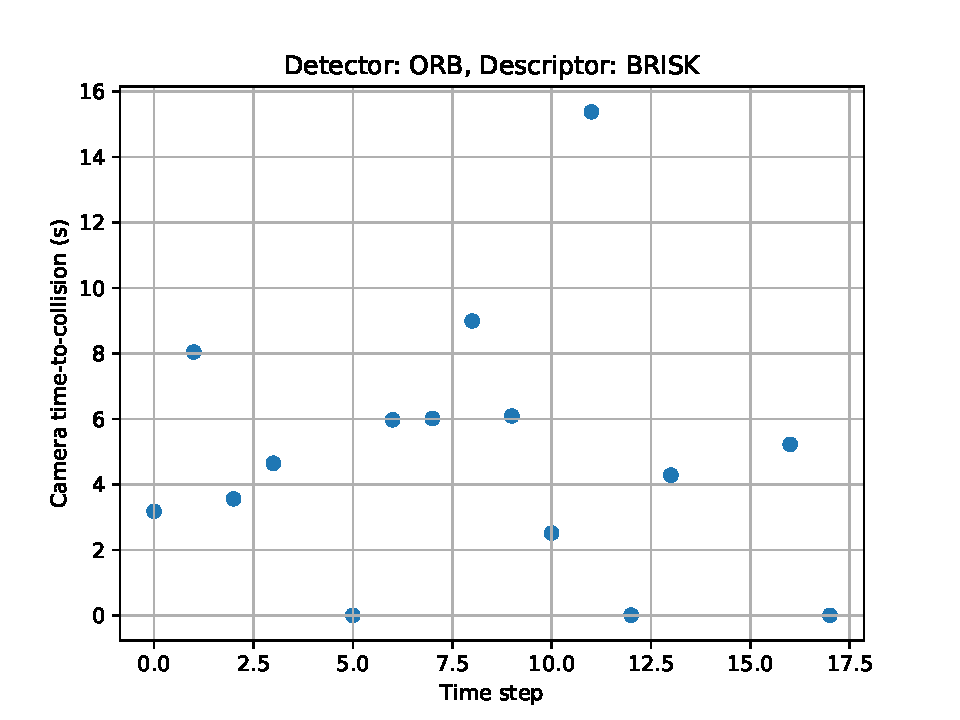
\includegraphics[width=\textwidth]{%
			./img/camera_ttc_det_ORB_desc_BRISK}
	\end{subfigure}
	\begin{subfigure}[c]{0.45\columnwidth}
		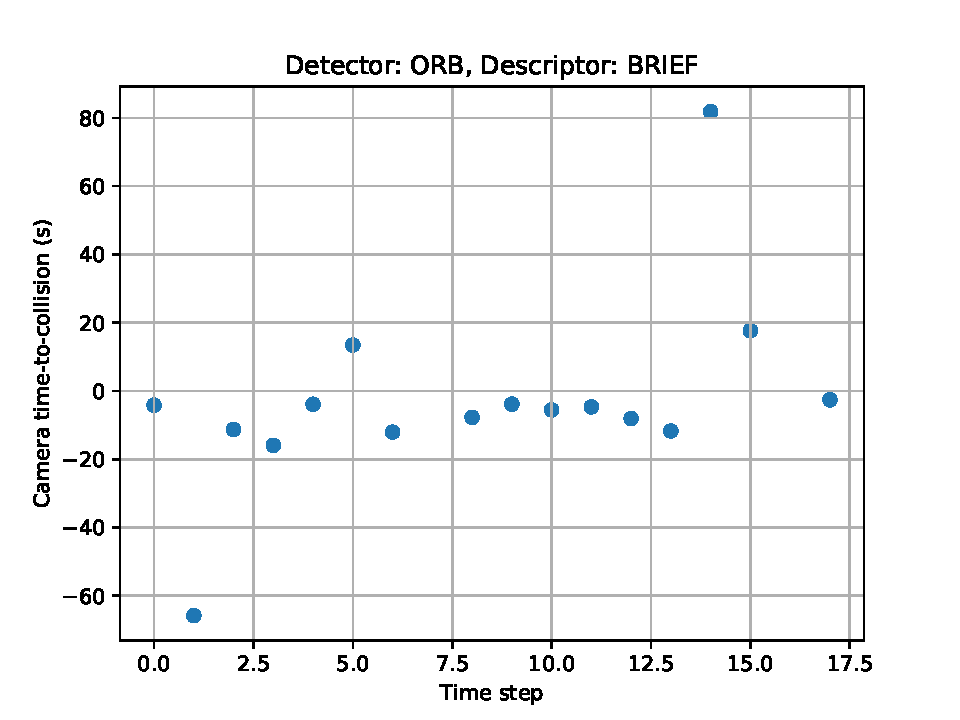
\includegraphics[width=\textwidth]{%
			./img/camera_ttc_det_ORB_desc_BRIEF}
	\end{subfigure}
	\begin{subfigure}[c]{0.45\columnwidth}
		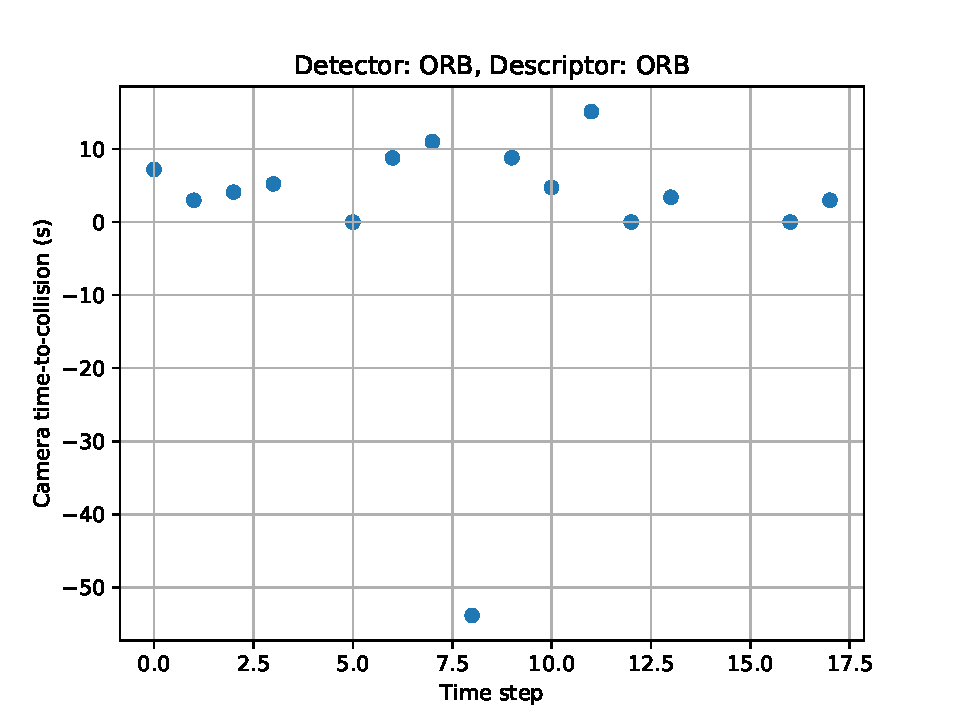
\includegraphics[width=\textwidth]{%
			./img/camera_ttc_det_ORB_desc_ORB}
	\end{subfigure}
	\begin{subfigure}[c]{0.45\columnwidth}
		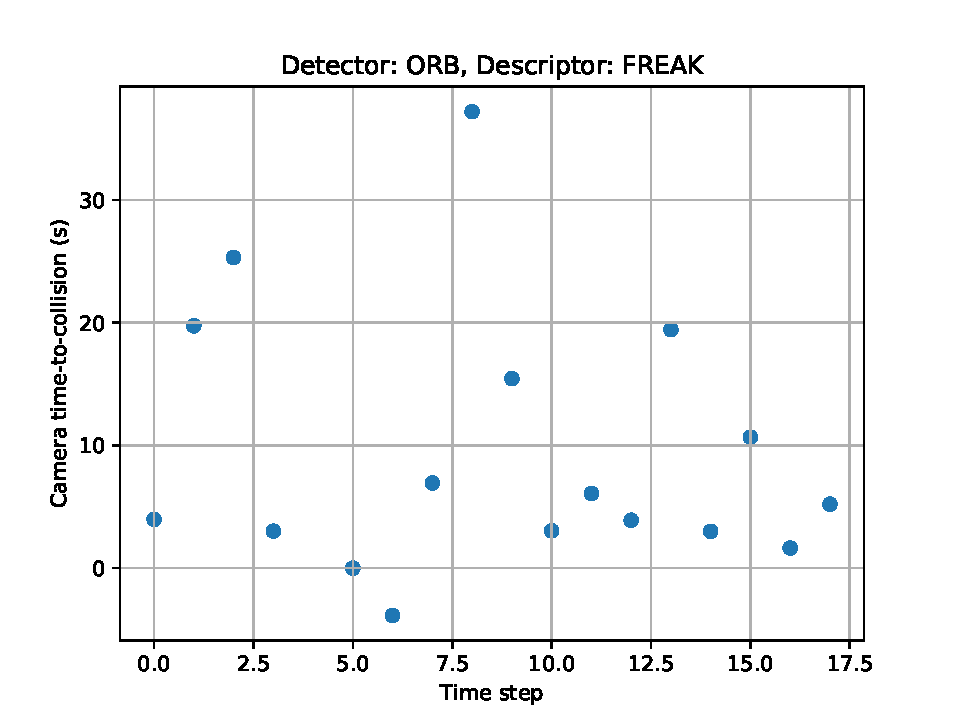
\includegraphics[width=\textwidth]{%
			./img/camera_ttc_det_ORB_desc_FREAK}
	\end{subfigure}
	\begin{subfigure}[c]{0.45\columnwidth}
		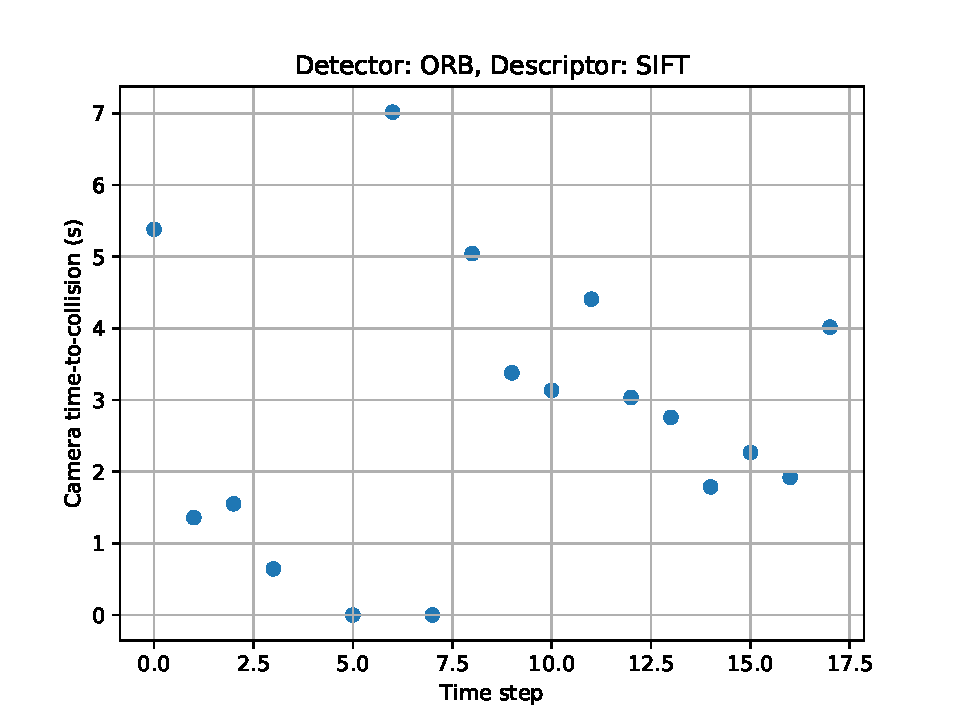
\includegraphics[width=\textwidth]{%
			./img/camera_ttc_det_ORB_desc_SIFT}
	\end{subfigure}
	\caption{Camera TTC for the ORB detector.}
	\label{fig:camera:ttc:detector_ORB}
\end{figure}

\begin{figure}
	\centering
	\begin{subfigure}[c]{0.45\columnwidth}
		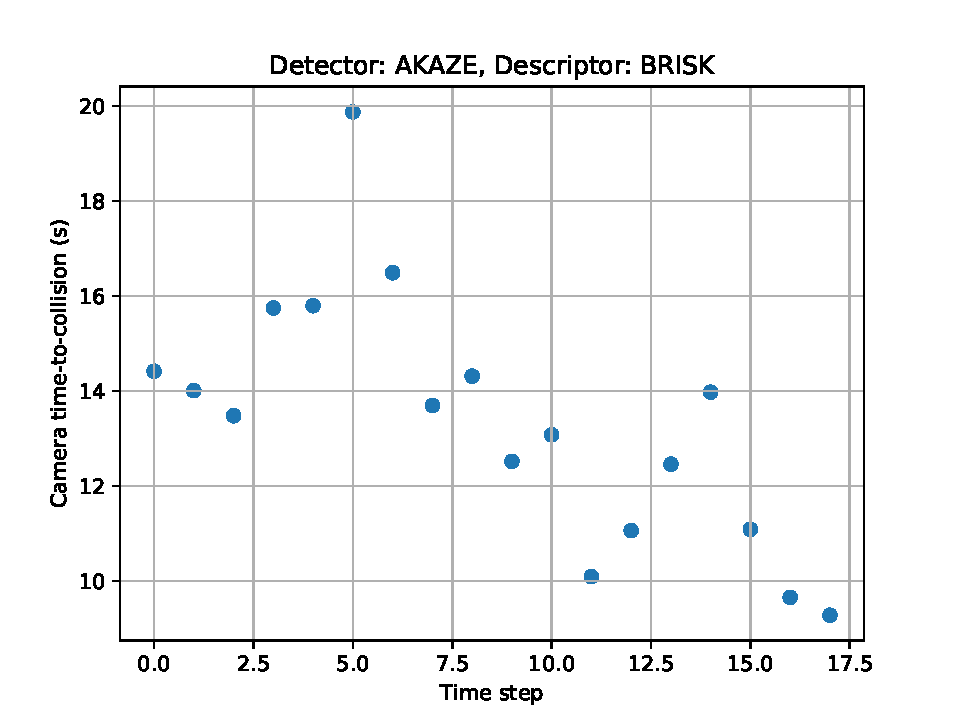
\includegraphics[width=\textwidth]{%
			./img/camera_ttc_det_AKAZE_desc_BRISK}
	\end{subfigure}
	\begin{subfigure}[c]{0.45\columnwidth}
		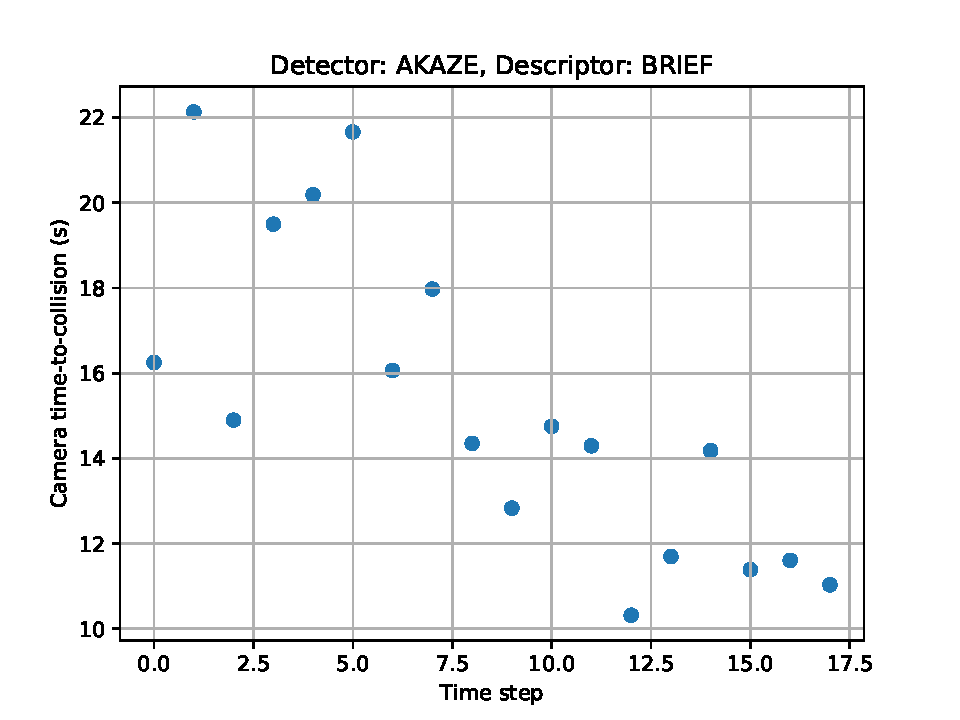
\includegraphics[width=\textwidth]{%
			./img/camera_ttc_det_AKAZE_desc_BRIEF}
	\end{subfigure}
	\begin{subfigure}[c]{0.45\columnwidth}
		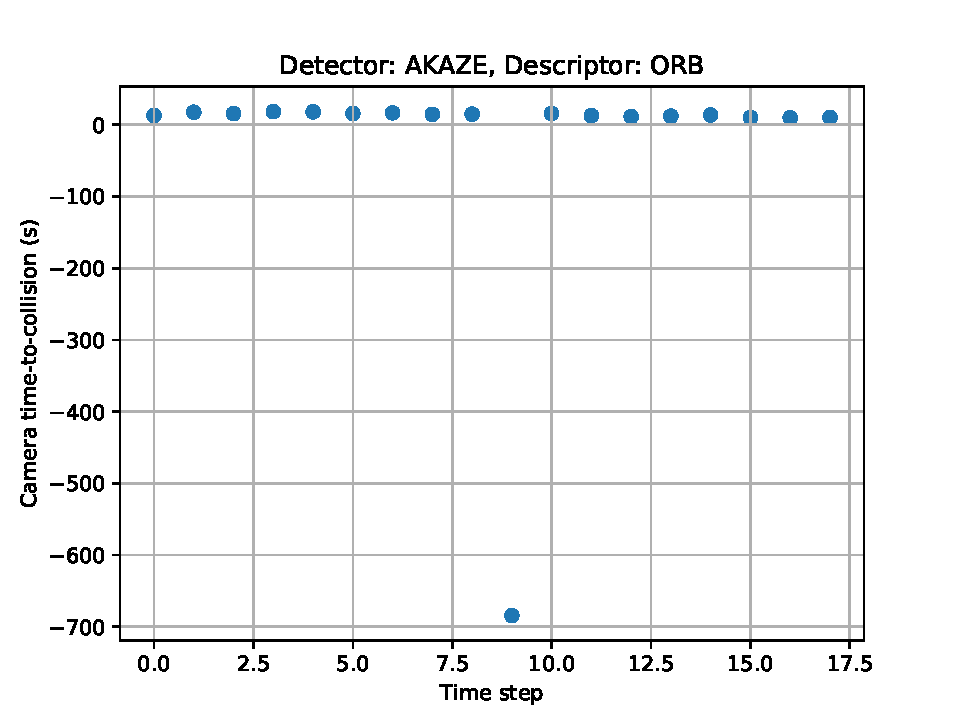
\includegraphics[width=\textwidth]{%
			./img/camera_ttc_det_AKAZE_desc_ORB}
	\end{subfigure}
	\begin{subfigure}[c]{0.45\columnwidth}
		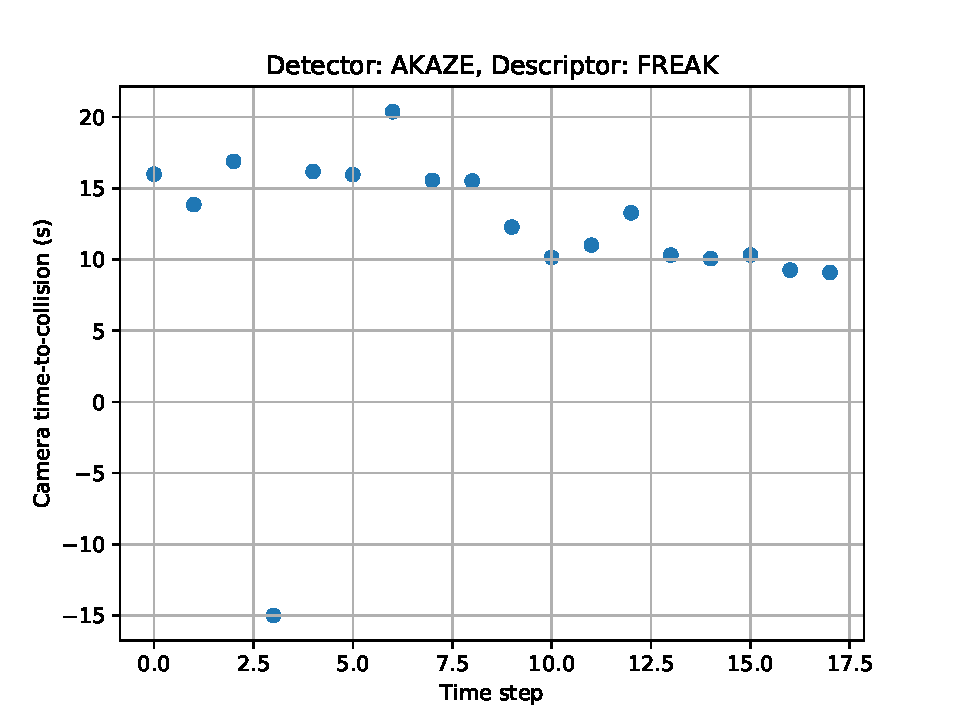
\includegraphics[width=\textwidth]{%
			./img/camera_ttc_det_AKAZE_desc_FREAK}
	\end{subfigure}
	\begin{subfigure}[c]{0.45\columnwidth}
		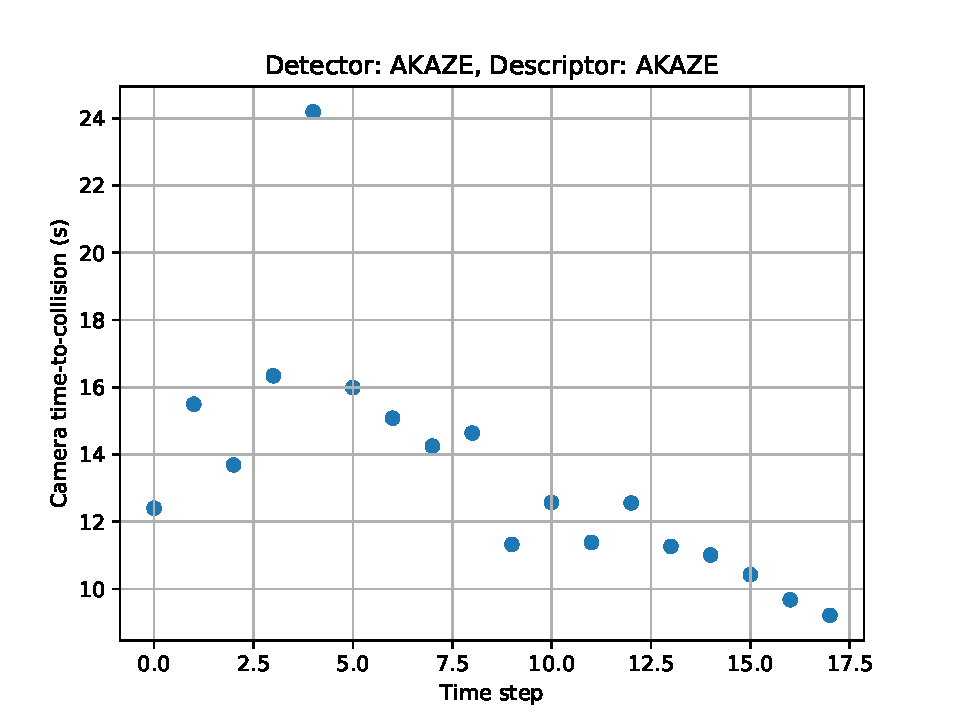
\includegraphics[width=\textwidth]{%
			./img/camera_ttc_det_AKAZE_desc_AKAZE}
	\end{subfigure}
	\begin{subfigure}[c]{0.45\columnwidth}
		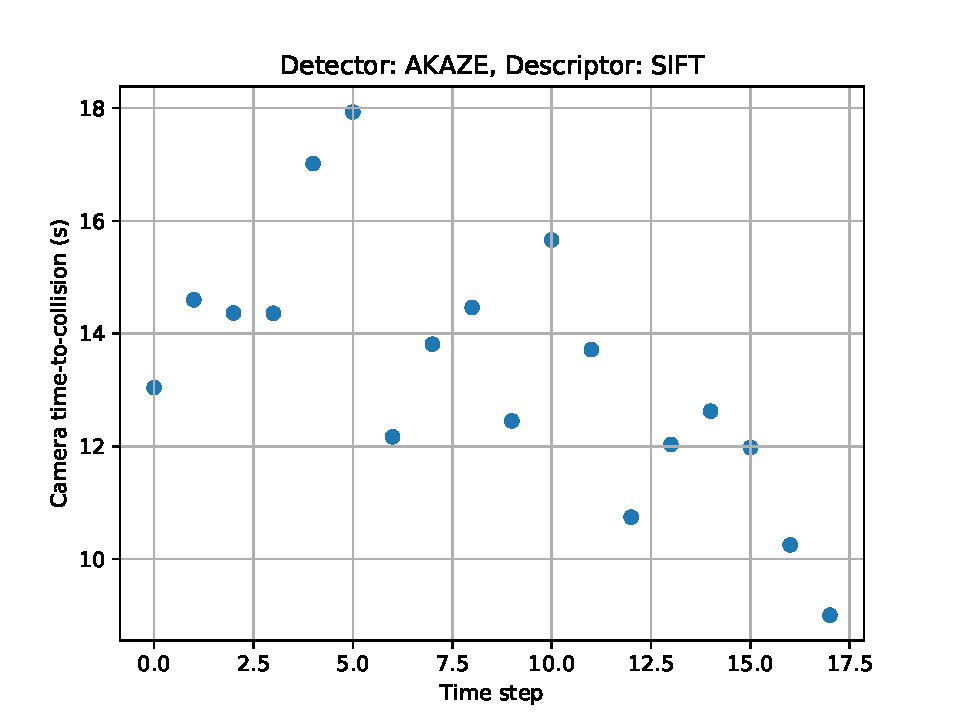
\includegraphics[width=\textwidth]{%
			./img/camera_ttc_det_AKAZE_desc_SIFT}
	\end{subfigure}
	\caption{Camera TTC for the AKAZE detector.}
	\label{fig:camera:ttc:detector_AKAZE}
\end{figure}

\begin{figure}
	\centering
	\begin{subfigure}[c]{0.45\columnwidth}
		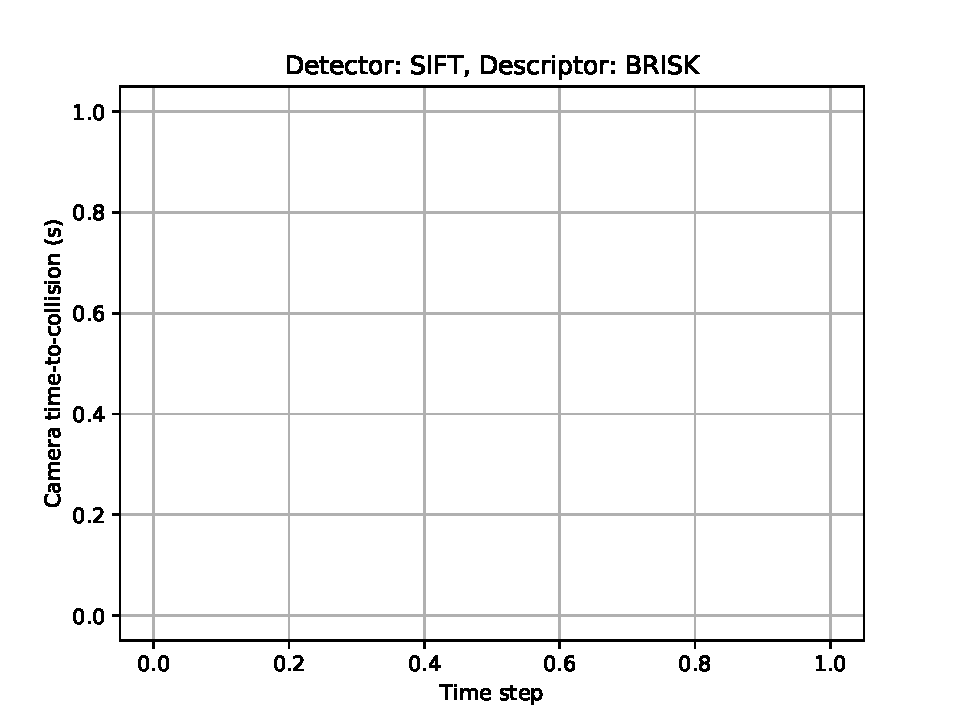
\includegraphics[width=\textwidth]{%
			./img/camera_ttc_det_SIFT_desc_BRISK}
	\end{subfigure}
	\begin{subfigure}[c]{0.45\columnwidth}
		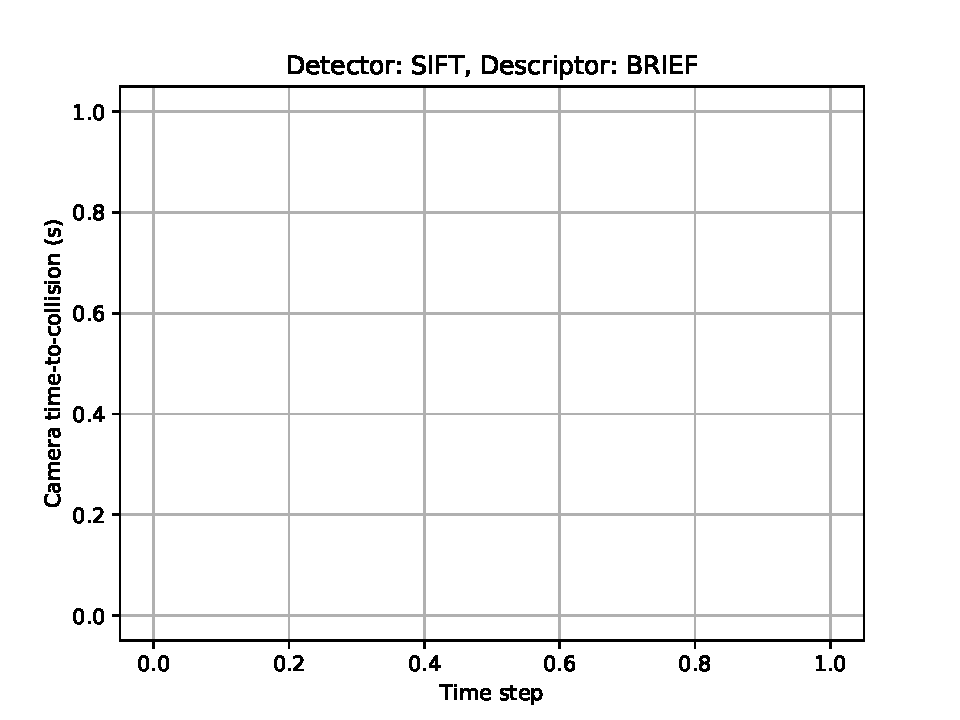
\includegraphics[width=\textwidth]{%
			./img/camera_ttc_det_SIFT_desc_BRIEF}
	\end{subfigure}
	\begin{subfigure}[c]{0.45\columnwidth}
		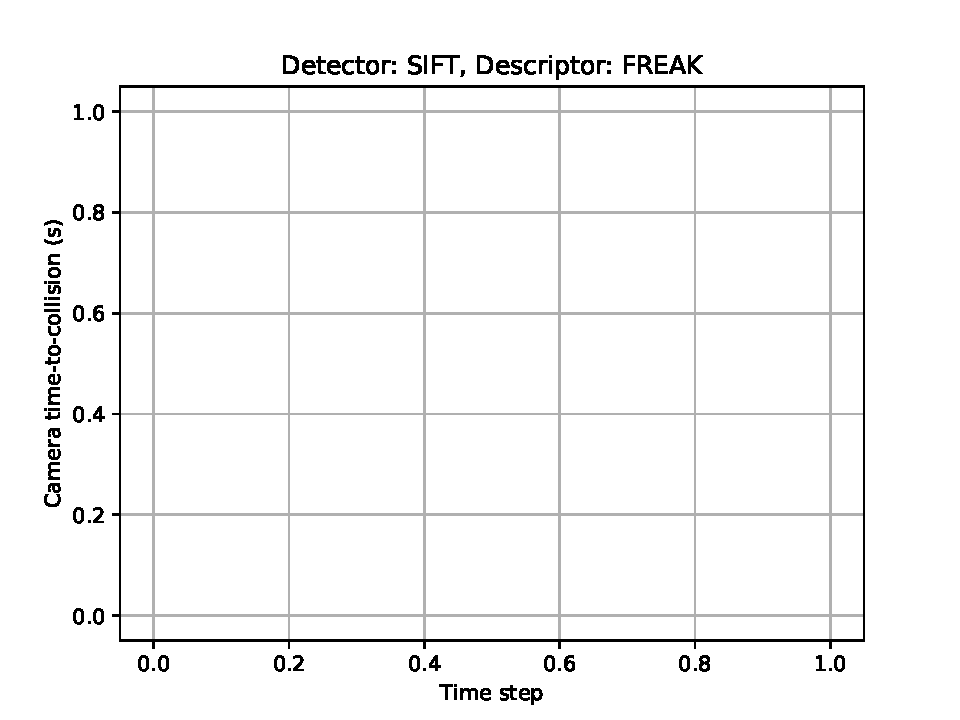
\includegraphics[width=\textwidth]{%
			./img/camera_ttc_det_SIFT_desc_FREAK}
	\end{subfigure}
	\begin{subfigure}[c]{0.45\columnwidth}
		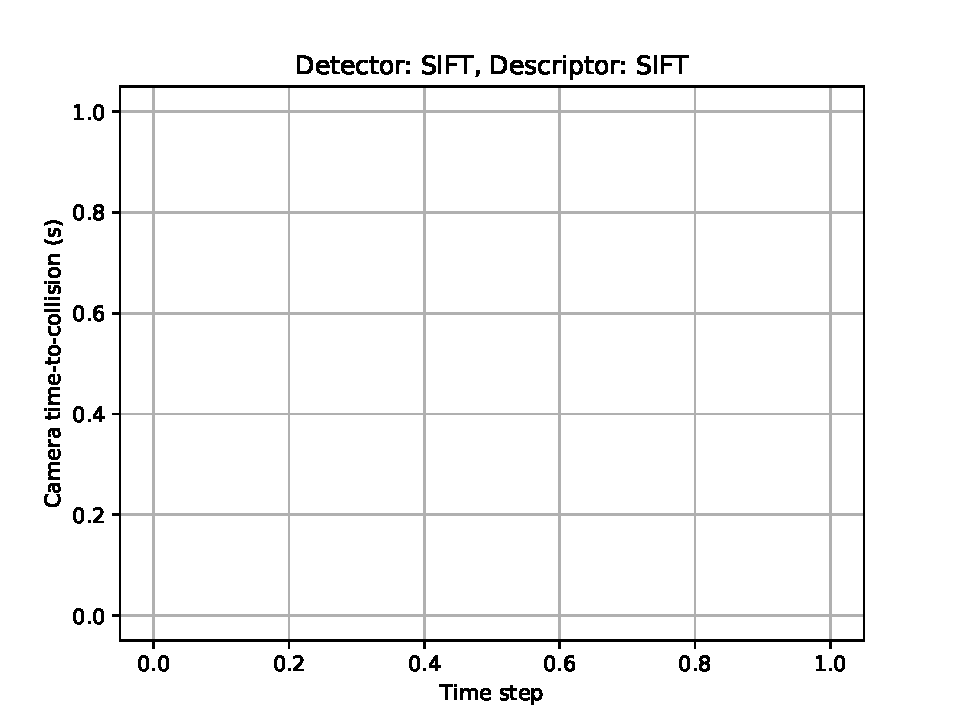
\includegraphics[width=\textwidth]{%
			./img/camera_ttc_det_SIFT_desc_SIFT}
	\end{subfigure}
	\caption{Camera TTC for the SIFT detector.}
	\label{fig:camera:ttc:detector_SIFT}
\end{figure}


\begin{table}
	\caption{Mean values and standard deviation for the ECT in seconds.
		The rows are the detectors,
		and the columns are the descriptors.}
	\label{tab:camera:etc_mean_and_std}
	\begin{tabular}{l|l||r|r|r|r|r|r}
		 			&      & BRISK & BRIEF & ORB & FREAK & AKAZE & SIFT	\\
		\hline \hline
		SHITOMASI 	& $\mu$ & 12.3164 & 10.8412 & 11.5964 & 6.95721 & N/A & 13.3082 \\
		 			& $\sigma$ & 2.5886 & 8.73406 & 2.34092 & 12.6196 & N/A & 1.99947 \\ \hline
		HARRIS 		& $\mu$ & 29.5739 & 3.29687 & 58.1579 & -24.507 & N/A & -23.0387 \\
		 			& $\sigma$ & 55.2819 & 75.1791 & 148.966 & 109.502 & N/A & 99.4211 \\ \hline
		FAST 		& $\mu$ & 13.2524 & 18.8866 & 14.9198 & 15.7288 & N/A & 8.19293 \\
		 			& $\sigma$ & 5.48023 & 8.88155 & 4.51431 & 17.6802 & N/A & 58.3958 \\ \hline
		BRISK 		& $\mu$ & NaN & NaN & NaN & NaN & N/A & 12.1515 \\
		 			& $\sigma$ & NaN & NaN & NaN & NaN & N/A & 7.1678 \\ \hline
		ORB 			& $\mu$ & NaN & NaN & NaN & NaN & N/A & NaN \\
					& $\sigma$ & NaN & NaN & NaN & NaN & N/A & NaN \\ \hline
		AKAZE 		& $\mu$ & 14.2429 & 16.1344 & -23.8059 & 12.5731 & 14.2648 & 14.1947 \\
		 			& $\sigma$ & 2.32234 & 3.29111 & 164.653 & 7.36428 & 3.13008 & 1.95166 \\ \hline
		SIFT 		& $\mu$ & NaN & NaN & N/A & NaN & N/A & NaN  \\
		 			& $\sigma$ & NaN & NaN & N/A & NaN & N/A & NaN  \\
		\hline
	\end{tabular}
\end{table}

\end{document}
